%#BIBTEX pbibtex -kanji=utf8 User_manual_jra55_do_v1_5
%\RequirePackage[l2tabu,orthodox]{nag}

% document class
\documentclass[dvipdfmx]{elsarticle_mod}

%\usepackage{lineno}

% my package

\usepackage{amssymb,amsmath}
\usepackage{newtxtext,newtxmath}
\usepackage{graphicx}
\usepackage{siunitx}
\usepackage{threeparttable}
\usepackage{here}
\usepackage{geometry}
\usepackage{lscape}
\usepackage{color}
\usepackage[colorlinks=true,linkcolor=blue,citecolor=blue,urlcolor=cyan]{hyperref}
\usepackage[left]{lineno}
\modulolinenumbers[1]

%%%%%%%%%%%%%%%%%%%%%%%%%%%%%%%%%%%%%%%%%%%%%%%%%%%%%%%%%%%%%%
\newcommand*\patchAmsMathEnvironmentForLineno[1]{%
  \expandafter\let\csname old#1\expandafter\endcsname\csname #1\endcsname
  \expandafter\let\csname oldend#1\expandafter\endcsname\csname end#1\endcsname
  \renewenvironment{#1}%
     {\linenomath\csname old#1\endcsname}%
     {\csname oldend#1\endcsname\endlinenomath}}% 
\newcommand*\patchBothAmsMathEnvironmentsForLineno[1]{%
  \patchAmsMathEnvironmentForLineno{#1}%
  \patchAmsMathEnvironmentForLineno{#1*}}%
\AtBeginDocument{%
\patchBothAmsMathEnvironmentsForLineno{equation}%
\patchBothAmsMathEnvironmentsForLineno{align}%
\patchBothAmsMathEnvironmentsForLineno{flalign}%
\patchBothAmsMathEnvironmentsForLineno{alignat}%
\patchBothAmsMathEnvironmentsForLineno{gather}%
\patchBothAmsMathEnvironmentsForLineno{multline}%
}
%%%%%%%%%%%%%%%%%%%%%%%%%%%%%%%%%%%%%%%%%%%%%%%%%%%%%%%%%%%%%%
% Macrocode to know a modified word
\def\Update{\color{red}} %% modified word
\def\Done{\color{black}} %%
\newcommand{\update}[1]{\textcolor{red}{#1}}
\def\Updatetwo{\color{green}} %% modified word
\newcommand{\updatetwo}[1]{\textcolor{green}{#1}}
%%%%%%%%%%%%%%%%%%%%%%%%%%%%%%%%%%%%%%%%%%%%%%%%%%%%%%%%%%%%%%

% margin
\geometry{top=2cm, bottom=2cm, left=1.5cm, right=1.5cm, includefoot}

%\journal{Journal of \LaTeX\ Templates}
%\journal{Ocean Modelling}

%%%%%%%%%%%%%%%%%%%%%%%
%% Elsevier bibliography styles
%%%%%%%%%%%%%%%%%%%%%%%
%% To change the style, put a % in front of the second line of the current style and
%% remove the % from the second line of the style you would like to use.
%%%%%%%%%%%%%%%%%%%%%%%

%% Numbered
%\bibliographystyle{model1-num-names}

%% Numbered without titles
%\bibliographystyle{model1a-num-names}

%% Harvard
\bibliographystyle{model2-names.bst}\biboptions{authoryear}

%% Vancouver numbered
%\usepackage{numcompress}\bibliographystyle{model3-num-names}

%% Vancouver name/year
%\usepackage{numcompress}\bibliographystyle{model4-names}\biboptions{authoryear}

%% APA style
%\bibliographystyle{model5-names}\biboptions{authoryear}

%% AMA style
%\usepackage{numcompress}\bibliographystyle{model6-num-names}

%% `Elsevier LaTeX' style
%\bibliographystyle{elsarticle-num}
%%%%%%%%%%%%%%%%%%%%%%%

\begin{document}

%\linenumbers

\begin{frontmatter}

\title{User manual of JRA-55 based surface dataset for driving ocean--sea-ice models (JRA55-do)}

%% Group authors per affiliation:
\author[MRIaddress]{Hiroyuki~Tsujino\corref{mycorrespondingauthor}}
\cortext[mycorrespondingauthor]{Corresponding author}
\ead{htsujino@mri-jma.go.jp}
\author[MRIaddress]{L.~Shogo~Urakawa}
\author[MRIaddress]{Hideyuki~Nakano}
\author[NCARaddress]{R.~Justin~Small}
\author[NCARaddress]{Who~M.~Kim}
\author[NCARaddress]{Stephen~G.~Yeager}
\author[NCARaddress]{Gokhan~Danabasoglu}
\author[JAMSTECaddress]{Tatsuo~Suzuki}
\author[UBristoladdress]{Jonathan~L.~Bamber}
\author[Bergenaddress]{Mats~Bentsen}
\author[Kieladdress]{Claus~B\"{o}ning}
\author[FSUaddress]{Alexandra~Bozec}
\author[FSUaddress]{Eric~Chassignet}
\author[Rutgersaddress]{Enrique~Curchitser}
\author[SIMONadd4,SIMONadd3,SIMONadd2,SIMONadd1]{Fabio Boeira Dias}
\author[LLNLaddress]{Paul~J.~Durack}
\author[GFDLaddress]{Stephen~M.~Griffies}
\author[MRIaddress]{Yayoi~Harada}
\author[Bergenaddress,Ilicakaddress]{Mehmet~Ilicak}
\author[NOCaddress]{Simon~A.~Josey}
\author[MRIaddress]{Chiaki~Kobayashi}
\author[JMAaddress]{Shinya~Kobayashi}
\author[JAMSTECaddress]{Yoshiki~Komuro}
\author[NCARaddress]{William~G.~Large}
\author[Grenobleaddress1,Grenobleaddress2]{Julien~Le~Sommer}
\author[SIMONadd1,SIMONadd2,SIMONadd3,SIMONadd4]{Simon~J.~Marsland}
\author[CMCCaddress1,CMCCaddress2]{Simona~Masina}
\author[Kieladdress]{Markus~Scheinert}
\author[NAGOYAaddress]{Hiroyuki~Tomita}
\author[READINGaddress]{Maria~Valdivieso}
\author[JAMSTECaddress,UTOKYOaddress]{Dai~Yamazaki}
 
\address[MRIaddress]{JMA Meteorological Research Institute, Tsukuba, Japan}
\address[NCARaddress]{National Center for Atmospheric Research (NCAR), Boulder, CO, USA}
\address[JAMSTECaddress]{Japan Agency for Marine-Earth Science and Technology (JAMSTEC), Yokohama, Japan}
\address[UBristoladdress]{University of Bristol, Bristol, UK}
\address[Bergenaddress]{Uni Research Climate, Bjerknes Centre for Climate Research, Bergen, Norway}
\address[Kieladdress]{GEOMAR Helmholtz Centre for Ocean Research Kiel, Kiel, Germany}
\address[FSUaddress]{Center for Ocean-Atmospheric Prediction Studies (COAPS), Florida State University, Tallahassee, FL, USA}
\address[Rutgersaddress]{Rutgers University, New Brunswick, NJ, USA}
\address[SIMONadd4]{Institute for Marine and Antarctic Studies, University of Tasmania, Australia}
\address[SIMONadd3]{Antarctic Climate and Ecosystems Cooperative Research Centre, University of Tasmania, Australia} 
\address[SIMONadd2]{Centre of Excellence for Climate System Science, Australia}
\address[SIMONadd1]{CSIRO Oceans and Atmosphere, Australia}
\address[LLNLaddress]{Program for Climate Model Diagnosis and Intercomparison. Lawrence Livermore National Laboratory, Livermore, CA, USA}
\address[GFDLaddress]{NOAA Geophysical Fluid Dynamics Laboratory (GFDL), Princeton, NJ, USA}
\address[Ilicakaddress]{Eurasia Institute of Earth Sciences, Istanbul Technical University, Istanbul, Turkey}
\address[NOCaddress]{National Oceanography Centre (NOC), Southampton, UK}
\address[JMAaddress]{Japan Meteorological Agency, Tokyo, Japan}
\address[Grenobleaddress1]{CNRS, LGGE, F-38041 Grenoble, France}
\address[Grenobleaddress2]{Univ. Grenoble Alpes, LGGE, F-38041 Grenoble, France}
\address[CMCCaddress1]{Centro Euro-Mediterraneo sui Cambiamenti Climatici (CMCC), Bologna, Italy}
\address[CMCCaddress2]{Istituto Nazionale di Geofisica e Vulcanologia (INGV), Bologna, Italy}
\address[NAGOYAaddress]{Nagoya University, Nagoya, Japan}
\address[READINGaddress]{Reading University, Reading, UK}
\address[UTOKYOaddress]{University of Tokyo, Tokyo, Japan}
 
%% or include affiliations in footnotes:
%\author[mymainaddress,mysecondaryaddress]{Elsevier Inc}
%\ead[url]{www.elsevier.com}

%\author[mysecondaryaddress]{Global Customer Service\corref{mycorrespondingauthor}}
%\cortext[mycorrespondingauthor]{Corresponding author}
%\ead{htsujino@mri-jma.go.jp}
%\address[mymainaddress]{1600 John F Kennedy Boulevard, Philadelphia}

\begin{abstract}
 This document describes the usage of the surface data set based on the Japanese 55-year Reanalysis, or JRA-55, for driving ocean--sea-ice models (JRA55-do).
\end{abstract}

\end{frontmatter}

\tableofcontents

\section{Introduction}

The purpose of this document is to provide the information needed for using the surface dataset based on the Japanese 55-year Reanalysis, JRA-55 (\citeauthor{Kobayashi_et_al_2015}~\citeyear{Kobayashi_et_al_2015}; \citeauthor{Harada_et_al_2016}~\citeyear{Harada_et_al_2016}), for driving ocean-sea ice models (JRA55-do). In JRA55-do, the surface meteorological variables taken from JRA-55 are adjusted relative to reference datasets to improve the mean states and the long-term variability. \citet{Tsujino_et_al_2018} presents details on the adjustments applied to the raw JRA-55 data. This dataset has been developed with an aim to be incorporated in the framework of Coordinated Ocean-ice Reference Experiments \citep[COREs;][]{Griffies_et_al_2012} and CMIP6 Ocean Model Intercomparison Project \citep[OMIP;][]{Griffies_et_al_2016} by replacing the forcing dataset that is currently used, the CORE interannual forcing version 2 \citep[COREv2;][]{Large_and_Yeager_2009}. It has been successfully adopted as the forcing dataset in the framework of phase-2 of Ocean Model Intercomparison Project (OMIP-2). \citet{Tsujino_et_al_2020} evaluates the OMIP-2 framework by comparing OMIP-1 and OMIP-2 simulations from 11 state-of-the-science global ocean--sea-ice models forced by COREv2 and JRA55-do forcing datasets, respectively.

In the following, the contents of the dataset are explained in Section \ref{sec:dataset-details}. Recommended methods for driving ocean--sea-ice models using the JRA55-do dataset are presented in Section \ref{sec:protocols}. How to obtain and cite the dataset are explained in Section \ref{sec:availability-citation}.

Appendices present technical details: Appendix \ref{app:raw-processing} explains the processing of the raw JRA-55 data. Appendix \ref{app:air} presents formulas to compute properties of moist air that we advocate replacing those used by the current CORE/OMIP framework. Appendix \ref{app:version} presents the version history.


\section{Details of the dataset}
\label{sec:dataset-details}

\subsection{Dataset description}

The JRA55-do dataset consists of nine surface-atmospheric variables derived from JRA-55 and two runoff variables (liquid water and solid ice discharge from land) derived from several sources (Table \ref{tab:main_variables-latest}). All surface-atmospheric fields are derived from the forecast phase of JRA-55 on the model grid. They are mapped from the reduced TL319 to the normal TL319 grid as explained in Appendix \ref{app:interp}. The temporal coverage is 3-hourly from the 1st of January 1958 to the present (to be updated at least annually). The downward surface fluxes, (the downwelling short- and longwave radiation fluxes) and precipitation (rain and snow), are averaged over three hours. The first datum of each year is averaged from 00:00 to 03:00 GMT on the 1st of January. Other surface-atmospheric fields, namely, the air temperature, specific humidity, wind vectors (all at 10 m height: see Appendix \ref{app:shift} for the height shift of temperature and specific humidity), and sea level pressure, are 3-hourly instantaneous values starting at 00:00 GMT on the 1st of January of each year.

All variables except the sea level pressure are modified from their original fields by multiplicative or offsetting factors to fit the reference fields derived from observations or other datasets. The modification and adjustment procedures are explained in detail by \citet{Tsujino_et_al_2018}.

JRA-55 does not directly provide the river runoff from rivers and glaciers at river mouths. JRA55-do derives them from several sources and provides liquid water flux ($\mathtt{friver}$) and solid ice calving flux ($\mathtt{licalvf}$) separately. The solid ice calving flux might be used as input to iceberg models. The liquid runoff fields are obtained from a river-routing model forced by runoffs from the land-surface component of JRA-55 \citep{Suzuki_et_al_2018}. The runoffs from Greenland and Antarctica, which contain a significant solid runoff component, are taken from independent estimates that combine satellite observations of solid discharge with high-resolution climate models of runoff and surface processes. The daily runoff from Greenland for version 1.3 is based on the monthly climatology (1961$-$1990) of \citet{Bamber_et_al_2012} and the liquid-plus-solid runoff is represented as the liquid water runoff ($\mathtt{friver}$) because the separate components were not available. For time interpolation from monthly to daily data, a method to preserve monthly mean values introduced by \citet{Killworth_1996} is used. The daily runoff from Greenland for version 1.4 is based on the monthly runoff from 1958 to 2016 of \citet{Bamber_et_al_2018}. Time interpolation from monthly to daily data is linear. For the period before 1958 and after 2016, the monthly climatology from 1958 to 1962 and from 2012 to 2016 is used, respectively. The separate time series of daily liquid and solid runoff are now provided for Greenland. The runoff from Antarctica \citep{Depoorter_et_al_2013} is constant in time and the liquid water and solid ice runoffs are separated. Note that there has been a shift in the treatment of liquid and solid components between version 1.3.01 and 1.3.02. See the version history presented in Appendix \ref{app:version_1_3_2} and Table \ref{tab:river_v1_3_2} for details.


\subsection{Supplementary data}

The dataset also includes the following supplementary data summerized in Table \ref{tab:suppl_variables-latest}.

\subsubsection{Variables at the sea-surface}

The variables at the sea-surface are necessary for computing surface fluxes. In most ocean--sea-ice models, these variables are taken from their own solution. Thus, including a set of sea-surface variables is not prerequisite to a dataset for driving ocean--sea-ice models. However, to assist computation of surface fluxes without using ocean--sea-ice models, the observation-based data for the sea-surface variables are provided as part of the dataset. We included surface temperature derived from brightness temperature of JRA-55, sea-surface temperature from COBE-SST \citep{Ishii_et_al_2005}, sea-ice area fraction from both JRA-55 and COBE-SST, and surface oceanic current from the GlobCurrent dataset \citep{Rio_et_al_2014}. The surface oceanic current may be added to the time series of the wind vector of this dataset to approximately construct a time series of the absolute wind vector.

In most ocean--sea-ice model simulations uncoupled with atmospheric models, sea-surface salinity is restored to observational data to prevent model drifts. For this purpose, we provide monthly climatology of sea-surface salinity derived from World Ocean Atlas 2013 version 2 (\citeauthor{Zweng_et_al_2013}, \citeyear{Zweng_et_al_2013}; \citeauthor{Boyer_et_al_2015}, \citeyear{Boyer_et_al_2015}). This is computed as an average in the upper 10 m, thus it should be more appropriately understood as salinity at 5 m depth.


\subsubsection{Land-sea mask}

The land-sea mask for the atmospheric data on TL319 grid is based on the original land-sea mask of JRA-55. The original land-sea mask (land=1, sea=0) on the reduced TL319 grid is linearly interpolated in the zonal direction onto the normal latitude$-$longitude (TL319) grid. A grid point valued at 0.5 or less is determined as a sea point; otherwise, it is assigned to land. Then, inland seas and lakes such as the Caspian Sea and Lake Victoria are manually buried and designated as land. In the provided data, land and sea grids are set to zero and unity, respectively.


\subsubsection{Grid information}

The Earth's sphere is occupied by grid cells centered at the latitudes and longitudes provided in the data file for each variable. Cell boundaries are given by $\texttt{lat\_bnds}$ and $\texttt{lon\_bnds}$ variables contained in each file. Note that the grid spacing is different depending on the variable. Atmospheric variables derived from JRA-55 are put on TL319 grid ($\sim 0.5625^{\circ}$). River runoff data are equally spaced by 0.25$^{\circ}$, starting at 0.125$^{\circ}$ longitude and $-89.875^{\circ}$ latitude. Therefore, the longitude and latitude bounds are also equally spaced, starting at 0$^{\circ}$ longitude and $-90^{\circ}$ latitude. The areas of the cells are provided for the atmospheric variables (TL319; $\mathtt{areacella}$) and the river runoff variables ($0.25^{\circ}\,\times\,0.25^{\circ}$; $\mathtt{areacello}$).

\begin{table}[h]
\centering
\caption{Description of the JRA55-do dataset version 1.5. The main variables listed here as well as supplementary data listed on Table \ref{tab:suppl_variables-latest} can be obtained at https://esgf-node.llnl.gov/search/input4mips/. Data files are stored in netCDF format. Each file contains the annual 3-hourly and daily time-series of a single variable on the TL319 and $0.25^{\circ}\,\times\,0.25^{\circ}$ grid, for atmospheric variables and river runoff variables, respectively. Time-series are constructed for each year, including leap years. The first column describes the name assigned to each variable in the netCDF file. These names are taken from Climate Model Output Rewriter (CMOR). The fourth column gives the grid and the appropriate cell area in Table \ref{tab:suppl_variables-latest} to be applied to make area averages. The sixth column gives the time of the first datum in each file. The seventh column states whether the given field is an averaged property or a snapshot. Note that rain ($\texttt{prra}$) plus snow ($\texttt{prsn}$) equals the total precipitation and that liquid ($\texttt{friver}$) plus solid ($\texttt{licalvf}$) equals the total runoff. \label{tab:main_variables-latest}}
\begin{threeparttable}
\begin{tabular*}{17.5cm}{p{1.4cm}|p{3.3cm}|p{1.6cm}|p{2.5cm}|p{1.4cm}|p{1.5cm}|p{2.8cm}}
\hline
variable name & field & units & horizontal grid and cell area & realm & first data represents & frequency (average or snapshot) \\ \hline \hline
$\texttt{tas}$  &  10 m air temperature   & $\mathrm{K}$ & TL319 (0.5625$^{\circ}$), $\texttt{areacella}$ & atmos & 0:00 1 Jan & 3-hour, snapshot \\ \hline
$\texttt{huss}$ &  10 m specific humidity & $\mathrm{kg}\,\mathrm{kg}^{-1}$ & TL319 (0.5625$^{\circ}$), $\texttt{areacella}$ & atmos & 0:00 1 Jan & 3-hour, snapshot \\ \hline
$\texttt{uas}$  &  10 m eastward wind     & $\mathrm{m}\,\mathrm{s}^{-1}$ & TL319 (0.5625$^{\circ}$), $\texttt{areacella}$ & atmos & 0:00 1 Jan & 3-hour, snapshot \\ \hline
$\texttt{vas}$  &  10 m northward wind    & $\mathrm{m}\,\mathrm{s}^{-1}$ & TL319 (0.5625$^{\circ}$), $\texttt{areacella}$ & atmos & 0:00 1 Jan & 3-hour, snapshot \\ \hline
$\texttt{psl}$  &  sea level pressure     & $\mathrm{Pa}$ & TL319 (0.5625$^{\circ}$), $\texttt{areacella}$ & atmos & 0:00 1 Jan & 3-hour, snapshot \\ \hline
$\texttt{rsds}$ &  downward shortwave     & $\mathrm{W}\,\mathrm{m}^{-2}$ & TL319 (0.5625$^{\circ}$), $\texttt{areacella}$ & atmos & 1:30 1 Jan & 3-hour, mean \\ \hline
$\texttt{rlds}$ &  downward longwave      & $\mathrm{W}\,\mathrm{m}^{-2}$ & TL319 (0.5625$^{\circ}$), $\texttt{areacella}$ & atmos & 1:30 1 Jan & 3-hour, mean \\ \hline
$\texttt{prra}$ & rainfall flux   & $\mathrm{kg}\,\mathrm{m}^{-2}\,\mathrm{s}^{-1}$ & TL319 (0.5625$^{\circ}$), $\texttt{areacella}$ & atmos & 1:30 1 Jan & 3-hour, mean \\ \hline
$\texttt{prsn}$ & snowfall flux   & $\mathrm{kg}\,\mathrm{m}^{-2}\,\mathrm{s}^{-1}$ & TL319 (0.5625$^{\circ}$), $\texttt{areacella}$ & atmos & 1:30 1 Jan & 3-hour, mean \\ \hline \hline
$\texttt{friver}$ & liquid water runoff\tnote{1} & $\mathrm{kg}\,\mathrm{m}^{-2}\,\mathrm{s}^{-1}$ & $0.25^{\circ}\,\times\,0.25^{\circ}$, $\texttt{areacello}$ & land & 1 Jan & day, mean \\ \hline
$\texttt{licalvf}$ & solid ice runoff represented as calving flux\tnote{2} & $\mathrm{kg}\,\mathrm{m}^{-2}\,\mathrm{s}^{-1}$ & $0.25^{\circ}\,\times\,0.25^{\circ}$, $\texttt{areacello}$ & landIce & 1 Jan & day, mean \\ \hline
\end{tabular*}
\begin{tablenotes}
\item[1]{Data of river discharge to the ocean \citep{Suzuki_et_al_2018} and liquid water runoffs around Greenland \citep{Bamber_et_al_2018} and Antarctica \citep{Depoorter_et_al_2013} are merged.}
\item[2]{Data of solid ice discharge to the ocean from Greenland \citep{Bamber_et_al_2018} and Antarctica \citep{Depoorter_et_al_2013} are merged.} 
\end{tablenotes}
\end{threeparttable}
\end{table}

\begin{table}[h]
\centering
\caption{Description of the supplementary data of JRA55-do. The first column describes the name assigned to each variable in the netCDF file. These names are taken from CMOR. \label{tab:suppl_variables-latest}}
\begin{threeparttable}
\begin{tabular*}{17.5cm}{p{1.6cm}|p{3.3cm}|p{1.4cm}|p{2.5cm}|p{1.4cm}|p{1.5cm}|p{2.8cm}}
\hline
variable name & field & units & horizontal grid and cell area & realm & first data represents & frequency (average or snapshot) \\ \hline \hline
$\texttt{ts}$   & brightness temperature from JRA-55 & $\mathrm{K}$  & TL319 (0.5625$^{\circ}$), $\texttt{areacella}$ & atmos & 0:00 1 Jan & 3-hour, snapshot \\ \hline
$\texttt{siconca}$ & sea-ice distribution from JRA-55 (0\% or 100\%) & \% & TL319 (0.5625$^{\circ}$), $\texttt{areacella}$ & seaIce & 0:00 1 Jan & 3-hour, snapshot \\ \hline
$\texttt{tos}$     & sea-surface temperature from COBE-SST \citep{Ishii_et_al_2005} & $\mathrm{^{\circ}C}$ & 1$^{\circ} \, \times \, 1^{\circ}$,  n/a & ocean & 1 Jan & day, mean \\ \hline
$\texttt{siconc}$  & sea-ice distribution from COBE-SST \citep{Ishii_et_al_2005} & \% & 1$^{\circ} \, \times \, 1^{\circ}$, n/a & seaIce & 1 Jan & day, mean \\ \hline
$\texttt{sos}$ & sea-surface salinity from World Ocean Atlas 2013 v2  (\citeauthor{Zweng_et_al_2013}, \citeyear{Zweng_et_al_2013}; \citeauthor{Boyer_et_al_2015}, \citeyear{Boyer_et_al_2015}) & 0.001 & $0.25^{\circ}\,\times\,0.25^{\circ}$, $\texttt{areacello}$ & ocean & - & month, climatology \\ \hline
$\texttt{uos}$ & sea water X velocity from GlobCurrent \citep{Rio_et_al_2014} & $\mathrm{m}\,\mathrm{s}^{-1}$ & TL319 ($0.5625^{\circ}$), $\texttt{areacella}$ & ocean & - & year, climatology \\ \hline
$\texttt{vos}$ & sea water Y velocity from GlobCurrent \citep{Rio_et_al_2014} & $\mathrm{m}\,\mathrm{s}^{-1}$ & TL319 ($0.5625^{\circ}$), $\texttt{areacella}$ & ocean & - & year, climatology \\ \hline \hline
$\texttt{areacella}$ & grid-cell area for surface atmospheric data & $\mathrm{m}^2$ & TL319 ($0.5625^{\circ}$), n/a & atmos & - & fixed \\ \hline
$\texttt{sftof}$ & Sea area percentage for surface atmospheric data (100\% for sea, 0\% for land) & \% & TL319 ($0.5625^{\circ}$), $\texttt{areacella}$ & atmos & - & fixed \\ \hline
$\texttt{areacello}$ & grid-cell area for liquid water ($\mathtt{friver}$) and solid ice ($\mathtt{licalvf}$) runoff data & $\mathrm{m}^{2}$ & $0.25^{\circ} \, \times, \, 0.25^{\circ}$, n/a & ocean & - & fixed \\ \hline
\end{tabular*}
\end{threeparttable}
\end{table}

\section{Recommended methods for driving ocean--sea-ice models using the JRA55-do dataset}
\label{sec:protocols}


It is basically recommended that the users follow the experimental protocol of OMIP \citep{Griffies_et_al_2016} for driving their ocean--sea-ice models using the JRA55-do dataset. Exception is the computation of properties of moist air, such as density, specific heat, latent heat of vaporization and sublimation of water vapor, and saturation specific humidity. We advocate using a set of formulas given by \citet{Gill_1982} for computing them, which is thought to be more accurate than the simple and cost-effective set of formulas used for the current CORE/OMIP framework as given by \citet{Large_and_Yeager_2004}. Appendix \ref{app:air} compares the two formulas.

After we accumulate experiences with the JRA55-do dataset for driving ocean--sea-ice models, we will provide recommendation on how ocean--sea-ice models should be suitably forced using this dataset.


\section{Dataset availability and citation}
\label{sec:availability-citation}

\subsection{How to obtain this dataset}

The dataset is registered with ``input datasets for Model Intercomparison Project (input4MIPs)'' and can be obtained from the input4MIPs website:\\
\hspace*{3zw}\texttt{https://esgf-node.llnl.gov/search/input4mips/}.\\
The dataset will be reached with searching keywords ``Target MIP'' = ``OMIP'', ``Institution ID'' = ``MRI'', and ``Source Version'' = ``1.5.0''.

Basic information about this dataset and an early release of the latest version waiting for publication at input4MIPs are available from the following:\\
\hspace*{3zw}\texttt{https://climate.mri-jma.go.jp/\~{}htsujino/jra55do.html}.\\
Note that we have started an automated extension of version 1.5.0 to the latest as v1.5.0.1 from March 2021 (the link to the dataset is provided in the above page), with some notable points given in Appendix \ref{app:version_1_5v2}.
%\hspace*{3zw}\texttt{https://climate.mri-jma.go.jp/\~{}htsujino/userspace/input4MIPs/CMIP6/OMIP/MRI/MRI-JRA55-do-1-5-0-1/jra55do_latest.html}.\\

The program codes used to generate the JRA55-do dataset can be obtained from a repository in Github:\\
\hspace*{3zw}\texttt{https://github.com/HiroyukiTsujino/JRA55-do/}.


\subsection{How to cite this dataset}
\label{sec:citation}

This dataset has been documented by \citet{Tsujino_et_al_2018}. The citing information for version 1.5 is given in the following:\\
\hspace*{3zw}\texttt{http://cera-www.dkrz.de/WDCC/meta/CMIP6/input4MIPs.CMIP6.OMIP.MRI.MRI-JRA55-do-1-5-0}.\\
To find the latest information on the dataset status and citation, please visit the living document:\\
\hspace{3zw}\texttt{http://goo.gl/r8up31}\\
or visit the following site, where the latest version will be available:\\
\hspace{3zw}\texttt{http://climate.mri-jma.go.jp/\~{}htsujino/jra55do.html}\\


For the convenience of the users of the earlier versions, the version history is presented in Appendix \ref{app:version}.

\appendix
\renewcommand{\thesection}{\Alph{section}}
\renewcommand{\thefigure}{\arabic{figure}}
\renewcommand{\thetable}{\arabic{table}}

\section{Processing raw JRA-55 data}
\label{app:raw-processing}

%
\subsection{Mapping from reduced to normal latitude$-$longitude (TL319) grid}
\label{app:interp}

The basic atmospheric model of JRA-55 uses a reduced TL319 grid, on which the raw JRA-55 data are provided. The number of longitudinal grid points is reduced at latitudes poleward of $41.5^{\circ}$, and the first datum of each latitude band is placed at 0$^{\circ}$ longitude.

After the first (main) adjustment stage, the adjusted data are zonally regridded at the common interval of 0.5625$^{\circ}$ for all latitude bands by the following rules:
\begin{itemize}
 \item If the target grid point is between two oceanic grid points, its value is found by linear interpolation.
 \item If the target grid point is between an ocean and a land grid point, it is treated as an ocean grid if it locates at the mid-point or closer to the ocean grid. Its value is then computed as the weighted average of the values of the ocean grid points among six candidate points. The candidate points are the three pairs of the two points flanking the target longitude or residing on the two adjacent latitudinal circles. The weighting factor is the inverse of the distance from the target point.
 \item If the target grid point is determined as a land point, its value is found by linear interpolation.
\end{itemize}


\subsection{Shifting the temperature and specific humidity of JRA-55 from 2 m to 10 m}

\label{app:shift}

JRA-55 provides the surface air temperature and specific humidity at 2 m above the surface. As in the CORE dataset, the temperature and specific humidity in the final dataset are provided at 10 m above the surface, where the wind vectors are measured. In JRA55-do, the air temperature and specific humidity of the JRA-55 forecast fields are adjusted at 2 m height, because the reference fields of both variables (IABP-NPOLES and the atmospheric reanalysis products for computing the ensemble mean) are available at this height. The main adjustments to the forecast fields are made on the original (reduced TL319) grid points of JRA-55.

After the main adjustment on the surface air temperature and specific humidity, the following steps are taken to produce the final product of the surface meteorological variables.
\begin{itemize}
 \item The equivalent neutral wind at 10 m height of JRA55-raw is estimated based on the adjusted air temperature and specific humidity at 2 m.
 \item The equivalent neutral wind field is adjusted.
 \item The adjusted air temperature and specific humidity at 2 m are shifted upwards to 10 m and the adjusted wind vector is converted from neutral to actual stability.
 \item Additional adjustments are performed on the air temperature and specific humidity at 10 m.
\end{itemize}

In the suite of operations, we use the bulk formula of \citet{Large_and_Yeager_2009} and a set of formulas to compute the properties of moist air based on \citet{Gill_1982} (Appendix \ref{app:air}). The surface temperatures of the ocean grids with and without sea-ice are taken from the surface brightness temperatures of JRA-55 and from COBE-SST, respectively. The surface temperatures of land grids are taken from the brightness temperature of JRA-55. The computation of the bulk transfer coefficient is iterated at most five times.

\section{Computation of properties of moist air}
\label{app:air}

In producing the JRA55-do dataset, a set of formulas given by \citet{Gill_1982} is used to compute properties of moist air, which is thought to be more accurate than that used for producing the CORE dataset. We recommend using these formulas for driving ocean--sea-ice models. Formulas used for producing the CORE dataset and in the current framework of CORE/OMIP are given by \citet{Large_and_Yeager_2004}, which is replicated here for comparison.

\subsection{Saturation specific humidity}

We consider computing saturation specific humidity in an environment with the sea-surface temperature $t$ ($^{\circ}\mathrm{C}$) and pressure $p$ ($\mathrm{hPa}$). The relation between the vapor pressure $e$ ($\mathrm{hPa}$) and specific humidity $q$ is given by
\begin{equation}
   e/p = q /(\omega + (1-\omega)q),
\end{equation}
where $\omega$ is the molecular weight ratio between water vapor and air:
\begin{equation}
 \omega = m_{\mathrm{w}}/m_{\mathrm{a}} = 18.016/28.966 = 0.62197.
\end{equation}
This is solved for the specific humidity as
\begin{equation}
   q = \omega e/(p - (1-\omega)e).
   \label{eq:def-specific_humidity}
\end{equation}

The relative humidity $\gamma$ is the mixing ratio of the mass of vapor to the mass of dry air divided by that of the saturated one. The mixing ratio ($r$) of the mass of vapor to the mass of dry air is given by
\begin{equation}
r = \frac{q}{1-q}.
\end{equation}
Thus, the relative humidity is computed using the specific humidity $q$ and the saturation specific humidity $q_{\mathrm{sat}}$ as
\begin{equation}
\gamma = \frac{q (1-q_{\mathrm{sat}})}{q_{\mathrm{sat}}(1-q)}.
\end{equation}

\subsubsection{Gill (1982)}

The saturation vapor pressure $e_{\mathit{sw}}$ (in units hPa) of pure water vapor over a plane water surface is given by
\begin{equation}
   \log_{10} e_{\mathit{sw}}(t) = (0.7859 + 0.03477\,t) / (1 + 0.00412\,t).
\end{equation}
In air, the partial pressure ${e'}_{\mathit{sw}}$ of water vapor at saturation is not exactly $e_{\mathit{sw}}$ but is given by
\begin{equation}
   {e'}_{\mathit{sw}} = f_{w} e_{\mathit{sw}}.
   \label{eq:partial_pressure_water}
\end{equation}
The value of $f_{w}$ is given by
\begin{equation}
   f_{w} = 1 + 10^{-6} p (4.5 + 0.0006 \, t^{2}),
   \label{eq:esat_correction}
\end{equation}
where $p$ is the pressure (units in hPa).

The saturation vapor pressure over a salt solution is less than over freshwater. For sea water, the reduction is about 2 \% (a factor of 0.98 should be applied to ${e'}_{\mathit{sw}}$).

The saturation vapor pressure $e_{\mathit{si}}$ of pure water vapor over ice is given by
\begin{equation}
   \log_{10} e_{\mathit{si}}(t) = \log_{10} e_{\mathit{sw}}(t) + 0.00422\,t.
   \label{eq:esat_ice_gill}
\end{equation}
The saturation partial pressure ${e'}_{\mathit{si}}$ in moist air is $f_{i}$ times $e_{\mathit{si}}$. Values of $f_{i}$ are given correct to 1 part in $10^{4}$ by (\ref{eq:esat_correction}). Thus
\begin{equation}
   {e'}_{\mathit{si}} = f_{w} e_{\mathit{si}}.
   \label{eq:partial_pressure_ice}
\end{equation}


\subsubsection{CORE}

Following \citet{Large_and_Yeager_2004}, over sea water,
\begin{equation}
q_{\mathrm{s}} = {\rho_a}^{-1} a_1 e^{a_2/(t+273.15)},
\label{eq:qsat_core}
\end{equation}
where $a_1 = 0.98 \times 640380 \,\mathrm{kg}\,\mathrm{m}^{-3}$ and $a_2 = -5107.4 \,\mathrm{K}$. The factor 0.98 applies only over sea-water. $\rho_a$ is the density of air. Over sea-ice, the formula of the same form is used, but now $a_1 = 11637800 \,\mathrm{kg}\,\mathrm{m}^{-3}$ and $a_2 = -5897.8 \,\mathrm{K}$. 

In summary, we advocate replacing the CORE computation of saturation specific humidity (\ref{eq:qsat_core}) with the more accurate formulation given by (\ref{eq:def-specific_humidity}) together with (\ref{eq:partial_pressure_water}) and (\ref{eq:partial_pressure_ice}).

\subsection{Specific heat}

The specific heat of air $c_{\mathit{pa}}$ is given as follows.

\subsubsection{Gill (1982)}

\begin{align}
c_{\mathit{pa}} &= \frac{7}{2} R \Big( 1 - q + \frac{8q}{7\omega} \Big), \nonumber \\ 
    &= 1004.6 \times (1 + 0.8735 q) \,(\mathrm{J}\,\mathrm{kg}^{-1}\,\mathrm{K}^{-1}).
\end{align}
Here, $R = 287.04\, \mathrm{J}\,\mathrm{kg}^{-1}\,\mathrm{K}^{-1}$ is the gas constant of dry air.

\subsubsection{CORE}

\begin{equation}
 c_{\mathit{pa}} = 1000.5 \,(\mathrm{J} \,\mathrm{kg}^{-1} \,\mathrm{K}^{-1}).
\end{equation}


\subsection{Latent heat}

The latent heat of vaporisation ($L_v$) and sublimation ($L_s$) are given as follows.

\subsubsection{Gill (1982)}

\begin{equation}
   L_v = 2.5008 \times 10^{6} - 2.3 \times 10^{3} t\, (\mathrm{J}\,\mathrm{kg}^{-1}),
   \label{ch9-eq:l_kr}
\end{equation}

\begin{equation}
   L_s = 2.839 \times 10^{6} - 3.6 (t + 35)^{2} \, (\mathrm{J}\,\mathrm{kg}^{-1}).
   \label{ch10-lasbl} 
\end{equation}

\subsubsection{CORE}

\begin{equation}
   L_v=2.5\times10^{6} \,(\mathrm{J}\,\mathrm{kg}^{-1}),
\end{equation}

\begin{equation}
   L_s=L_v+L_f=2.839\times10^{6} \,(\mathrm{J}\,\mathrm{kg}^{-1}).
\end{equation}
Here, $L_f$ is the latent heat of fusion:
\begin{equation}
   L_f = 3.337 \times 10^{5}  \,(\mathrm{J}\,\mathrm{kg}^{-1}).
\end{equation}

As \citet{Brodeau_et_al_2010} pointed out, choosing \citeauthor{Gill_1982}'s (\citeyear{Gill_1982}) formula will result in a smaller latent heat loss from the ocean than the case where a constant as in CORE is chosen. The surface heat flux budget will be positively biased (heating of the ocean) in comparison with the evaluation presented by \citet{Large_and_Yeager_2009}.


\subsection{Air density}

The equation of state of moist air of temperature $\theta$ (K) under the pressure $P$ (Pa) is given by
\begin{equation}
\rho_{a} = \frac{P}{R\theta(1-q+q/\omega)} \equiv P/R T_v,
\end{equation}
where
\begin{equation}
T_v \equiv \theta(1-q+q/\omega) = \theta (1+0.6078q)
\end{equation}
is called the virtual temperature.

\subsubsection{Gill (1982)}

\begin{equation}
\rho_{a} = \frac{P}{R\theta(1-q+q/\omega)}.
\end{equation}

\subsubsection{CORE}

\begin{equation}
\rho_{a} = 1.22 \,(\mathrm{kg}\, \mathrm{m}^{-3}).
\end{equation}


\section{Version history, bugs, and fixes}

\label{app:version}

As of September 2020, we maintain version 1.5. This version is planned to be continually updated to the present at least annually. The latest revision of version 1.5 will be provided as a self-contained dataset, that is, it will contain the full set of variables. The version will proceed, accompanied by a detailed document, when new datasets or adjustment methods are incorporated. 

There are several older versions which are listed below. Because there are many users of the older versions 1.1 and 1.2, we specifically list the fixes and upgrades included in versions 1.3 and 1.2 relative to their immediate predecessors as a reference for the users of those versions.

\subsection{JRA55-v0.1 (March 2015)}

Unadjusted JRA-55 (JRA55-v0.1) is produced in a format (e.g., grid, units, etc.) compatible with the adjusted version (JRA55-v0.2).

\subsubsection{JRA55-v0.1.01 (December 2015; Fix of short wave radiation)}

Because it was found that short wave radiation of JRA55-v0.1 was identical to the adjusted data set (JRA55-v0.2), the data files should be replaced with the correct (unadjusted) data.

\subsection{JRA55-v0.2 (March 2015)}

JRA55-v0.2 is released at the end of March, 2015, for close inspection by voluntary individuals and groups.


\subsection{JRA55-v0.3 and v0.4 (December 2015)}

\begin{itemize}
\item JRA55-v0.3 with a revised adjustment method is produced in preparation for the extend CLIVAR-OMDP meeting to be held in January 2016. 
\item JRA55-v0.4 cuts off extremely low temperature south of 60$^{\circ}$S of JRA55-v0.3 using the same lower limit used by the CORE data set.
\item The land-sea mask has been changed: The original land-sea mask (land=1, sea=0) on the reduced grid is interpolated on the normal latitude-longitude (TL319) grid by linear interpolation in the zonal direction. A grid point whose value is equal to or is less than 0.5 is determined to be sea, otherwise determined to be land.
\end{itemize}

\subsection{JRA55-v0.5,v0.6,v0.7}

These versions are for internal tests. They are not going to be published but are reflected in v0.8.

\subsection{JRA55-v0.8 (June 2016)}

The adjustment method is further revised. On the basis of shift in the quality of JRA-55, we set three periods for which different adjustment factors are applied.

\subsection{JRA55-do-v1.0 (November 2016)}

This is intended to be the first official version. Relative to JRA55-v0.8, new river runoff data sets are added. Precipitation (rain and snow) is slightly changed globally to achieve a surface fresh water flux balance with the new river runoff. Other elements are unchanged.


\subsection{JRA55-do-v1.1 (December 2016)}

To follow up the requests on the change in the format of the river data and to correct minor bugs in the processing of river data for version 1.0, the river runoff as well as precipitation (rain and snow) of version 1.0 have been updated. For precipitation, as in version 1.0, the spatial structure and temporal variability of precipitation of version 0.8 (JRA55-v0.8) have been retained. One may render the JRA55-v0.8 precipitation to that of version 1.1 by applying a constant factor of $\frac{1.020163}{1.024288} \sim 0.9959728$ (about 0.4 \% reduction) to the precipitation of JRA55-v0.8. JRA55-do-v1.1 has been updated to the early 2018 and is available from the following:\\
\hspace*{3zw} \texttt{http://amaterasu.ees.hokudai.ac.jp/\~{}tsujino/JRA55-do-v1.1/}.\\
Note that variable names are different relative to those used for the latest version explained in Section \ref{sec:dataset-details}. No further update is planned for this version. Users are recommended to shift to the latest version.



\subsection{JRA55-do-v1.2 (September 2017)}

\label{app:version_1_2}

Version 1.2 includes the following updates relative to version 1.1.
\begin{itemize}
\item (Bug fix) Error in computing the annual mean climatology of wind speed for JRA-55 and JRA-55C was corrected. This resulted in the minor changes in the adjustment factors for wind speed. They were less than 0.5 \%.
\item (Bug fix) Temperature and specific humidity anomaly of CORE relative to JRA-55 were not added to JRA-55 in inland seas and lakes poleward of 40$^{\circ}$N.
\item (Upgrade) Phase-III for precipitation adjustment is further divided into 1999$-$2006 and 2006$-$2015 to suppress recent increasing trend.
\item (Upgrade) Contributions to temperature and specific humidity reference data (ensemble mean) from NCEP-R1, NCEP-R2, and 20CRv2 were weakened around semi-enclosed seas.
\item (Upgrade) Region of full ice-cover (>0.99) used for smoothing temperature and specific humidity was determined based on daily, instead of monthly, COBE-SST data to facilitate quicker updating in the future.
\item (Upgrade) In calculating surface fluxes using the bulk formula to determine the globally uniform, constant adjustment factors applied to downward fluxes, scalar wind speed is first calculated on the original grid of the dataset and then interpolated on COBE-SST (1$^{\circ} \times 1^{\circ}$) grid. In the older treatment, components of wind vector are interpolated on COBE-SST grid first, and then scalar wind is computed.
\end{itemize}

Figure \ref{fig:waterflux_v1_1} shows the comparison of surface fresh water fluxes between versions 1.1 and 1.2. The global ocean averaged evaporations of versions 1.1 and 1.2 are almost identical (overwrapped), but that of version 1.1 is reduced by about 1 \% when the older treatment on wind is applied (the last item in the above list). This is reflected in the smaller precipitation of version 1.1 before 1996 (phases I and II), when the common spatially dependent adjustment factors are used between versions 1.1 and 1.2. In version 1.1 that did not divide the adjustment period for phase-III (1999-present), the precipitation shows an increasing trend in the most recent decade. This motivated us to divide phase-III at 2006, when GNSS-RO as well as the increased number of radiance observations from satellite water vapor channels are introduced.

Because of the quick transition to the next version (v1.3), this version is not made widely available.

\begin{figure}[h]
\centering
  \resizebox{12cm}{!}{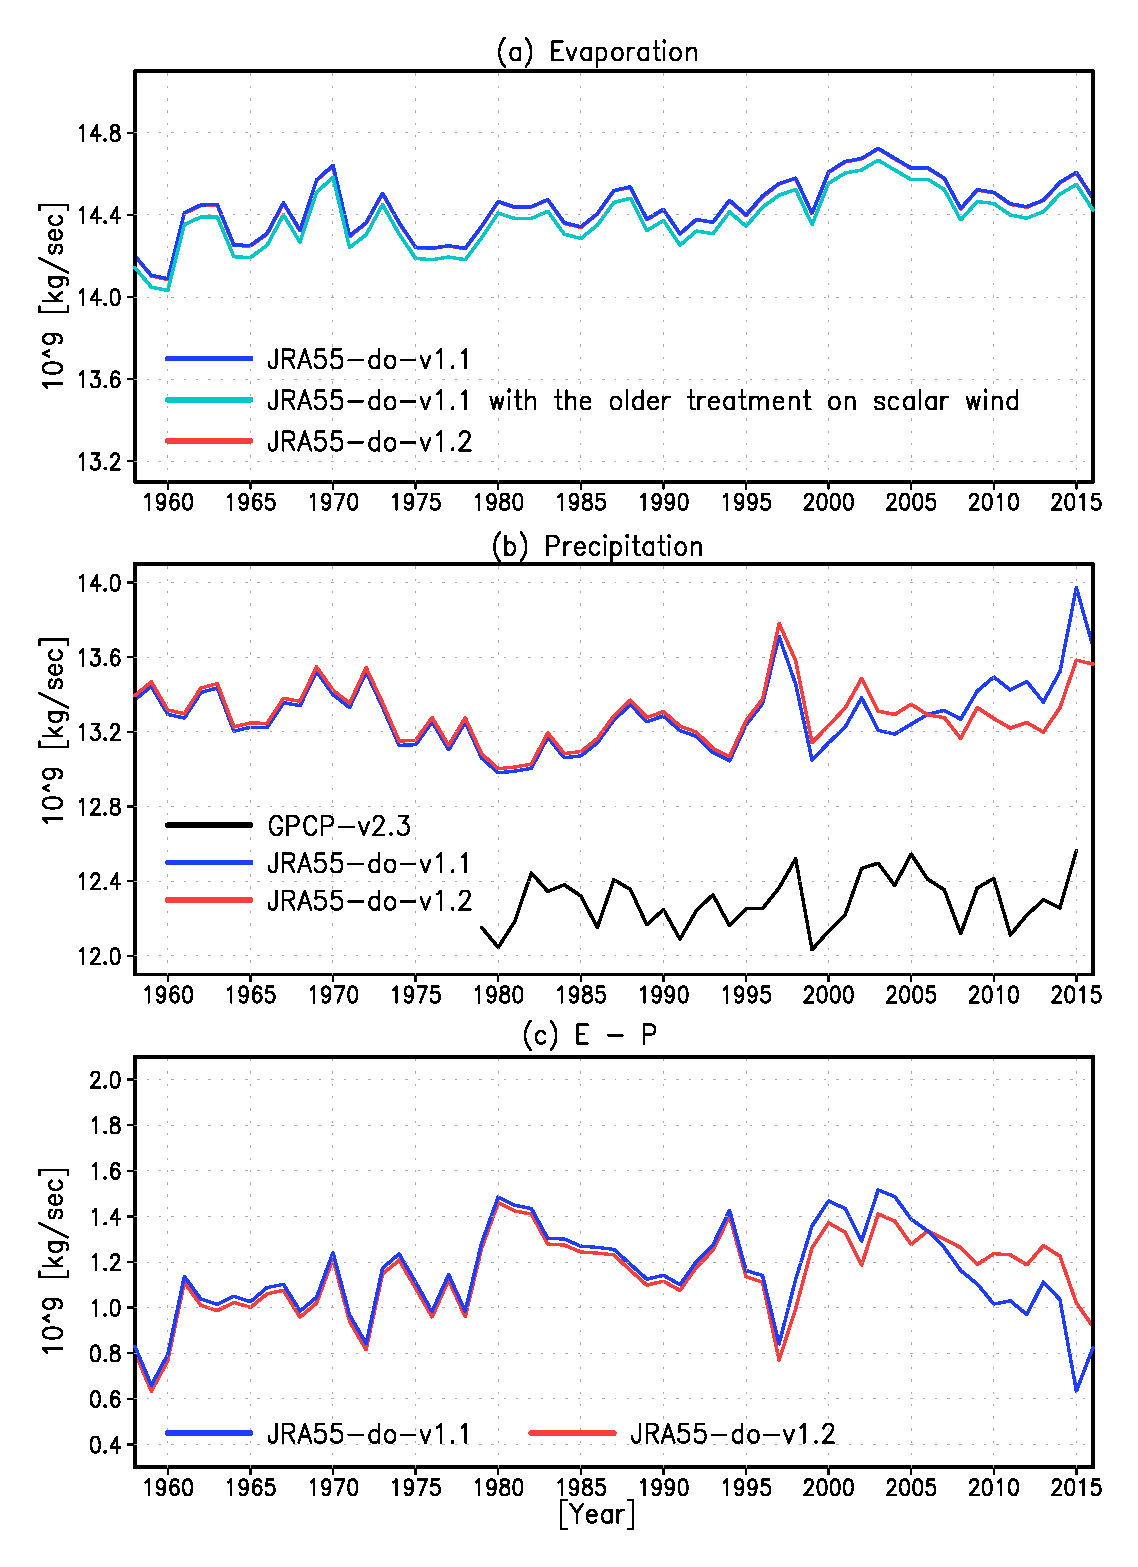
\includegraphics{waterflux_jra55_v1_1_v1_2.eps}}
 \caption{(a) Time-series of the annual mean global ocean integrated (a) evaporation, (b) precipitation, (c) evaporation minus precipitation ($\times 10^{9}\,\mathrm{kg}\, \mathrm{s}^{-1}$) of JRA55-do-v1.1 (blue), and JRA55-do-v1.2 (red). Light blue line in (a) is the evaporation using the older treatment of scalar wind speed (see text). In (a), the blue (v1.1) and the red (v1.2) lines are almost overwrapped. Black line in (b) is the precipitation of GPGP v2.3. Bulk formula and air-properties formulas are taken from \citet{Large_and_Yeager_2009} and \citet{Gill_1982}, respectively.}
  \label{fig:waterflux_v1_1}
\end{figure}

\subsection{JRA55-do-v1.3 (December 2017)}

\label{app:version_1_3}

In version 1.2, the magnitude of the wind vector was adjusted by a multiplicative factor $R_{\mathrm{S}}(\lambda,\phi)$, whereas an offset factor was used for version 1.3. The adjustment on the wind direction is done using a counter-clockwise offset factors $\chi(\lambda,\phi)$. These adjustment factors are constant in time. In version 1.2, the wind vector of JRA55-raw ($u_{\mathrm{JRA55}}$, $v_{\mathrm{JRA55}}$) at ($\lambda$,$\phi$) was adjusted as follows:
\begin{equation}
  \left(
    \begin{array}{c}
      u_{\mathrm{adj}} \\
      v_{\mathrm{adj}} 
    \end{array}
  \right)
  =
  R_{\mathrm{S}}(\lambda,\phi) \, \left(
    \begin{array}{rr}
      \cos \chi & -\sin \chi \\
      \sin \chi & \cos \chi
    \end{array}
  \right)
  \left(
    \begin{array}{c}
      u_{\mathrm{JRA55}} \\
      v_{\mathrm{JRA55}}
    \end{array}
  \right),
\end{equation}
where
\begin{equation}
  R_{\mathrm{S}} = \frac{\bar{W}_{\mathrm{ref}}}{\bar{W}_{\mathrm{JRA55}}}. \label{eq:windadj-v1-2}
\end{equation}
As shown in (\ref{eq:windadj-v1-2}), the multiplicative factor ($R_{\mathrm{S}}$) was determined as the ratio of the long-term average the reference wind speed $(\bar{W}_{\mathrm{ref}})$ to that of JRA55-raw $(\bar{W}_{\mathrm{JRA55}})$, where
\begin{equation}
   W_{\mathrm{JRA55}} = \max\big(\sqrt{u^2_{\mathrm{JRA55}}+v^2_{\mathrm{JRA55}}},\,\, 0.3\, \mathrm{m}\,\mathrm{s}^{-1}\big).
 \label{eq:floor-wind}
\end{equation}

In this adjustment method, high winds are selectively modified by a large amount to give a mean wind speed that matches that of the reference field. This treatment may significantly modify the variance of the wind speed and hence the magnitude of the wind stress, which is quadratic of the wind speed.

Thus, in version 1.3, the magnitude of the wind vector was adjusted by an offset factor $\Delta W(\lambda,\phi)$, whereas a counter-clockwise offset factor $\chi(\lambda,\phi)$ was continually used for the direction. Specifically, the wind vector of JRA55-raw ($u_{\mathrm{JRA55}}$, $v_{\mathrm{JRA55}}$) at ($\lambda$,$\phi$) was adjusted as follows:
\begin{equation}
  \left(
    \begin{array}{c}
      u_{\mathrm{adj}} \\
      v_{\mathrm{adj}} 
    \end{array}
  \right)
  =
  \frac{W_{\mathrm{JRA55}} + c \Delta W}{W_{\mathrm{JRA55}}} \, \left(
    \begin{array}{rr}
      \cos \chi & -\sin \chi \\
      \sin \chi & \cos \chi
    \end{array}
  \right)
  \left(
    \begin{array}{c}
      u_{\mathrm{JRA55}} \\
      v_{\mathrm{JRA55}}
    \end{array}
  \right),
  \label{eq:wind-adjust}
\end{equation}
and
\begin{equation}
  c = \mathrm{tanh}(d),\,\,\,\, d = \frac{\max(W_{\mathrm{JRA55}} - 0.3\,(\mathrm{m}\,\mathrm{s}^{-1}),0)} {|\Delta W|}. \label{eq:taper-windcorrec}
\end{equation}
In (\ref{eq:wind-adjust}), the offset factors for the wind speed ($\Delta W$) were determined by comparing the long-term average of JRA55-raw $(\bar{W}_{\mathrm{JRA55}})$ with that of the reference wind speed $(\bar{W}_{\mathrm{ref}})$, and were quantified as the difference between the reference and JRA55-raw:
\begin{equation}
   \Delta W = \bar{W}_{\mathrm{ref}} - \bar{W}_{\mathrm{JRA55}}.
\end{equation}
In (\ref{eq:floor-wind}), \SI{0.3}{m.s^{-1}} floor on the neutral wind speed of JRA55-raw was introduced to avoid the zero division in (\ref{eq:wind-adjust}). The factor $c$ defined by (\ref{eq:taper-windcorrec}) tapers the adjustment to ensure that wind speed is not modified for the minimum wind speed ($W_\mathrm{JRA55}=0.3\,\mathrm{m}\,\mathrm{s}^{-1}$): Adjustment is not applied ($c=0$) for the minimum wind speed and gets closer to the full adjustment ($c=1$) as the wind gets higher.


Figures \ref{fig:taux_v1_3-v1_2} and \ref{fig:tauy_v1_3-v1_2} show the comparison of the basin-wide zonal mean wind stress. As expected, the zonal wind stresses (Figure \ref{fig:taux_v1_3-v1_2}) are enhanced in version 1.3 in the mid-latitude westerly region. The zonal wind stresses in the mid latitudes of the Northern Hemisphere get close to whereas those of the Southern Hemisphere get too strong relative to the Scatterometer Oceanic Wind Stress (SCOW) product \citep{Risien_and_Chelton_2008} in version 1.3. However, the Southern Ocean westerly in version 1.3 still exhibits improvement relative to JRA55-raw (Figure \ref{fig:comp_taux_basin}). The meridional wind stresses are similar between versions 1.2 and 1.3 (Figure \ref{fig:tauy_v1_3-v1_2}). As shown in Figures \ref{fig:comp_taux_basin} and \ref{fig:comp_tauy_basin}, version 1.3 is generally closer to SCOW than CORE and JRA55-raw. For these reasons, we made a shift to version 1.3.


\begin{figure}[h]
  \centering
  \resizebox{!}{15cm}{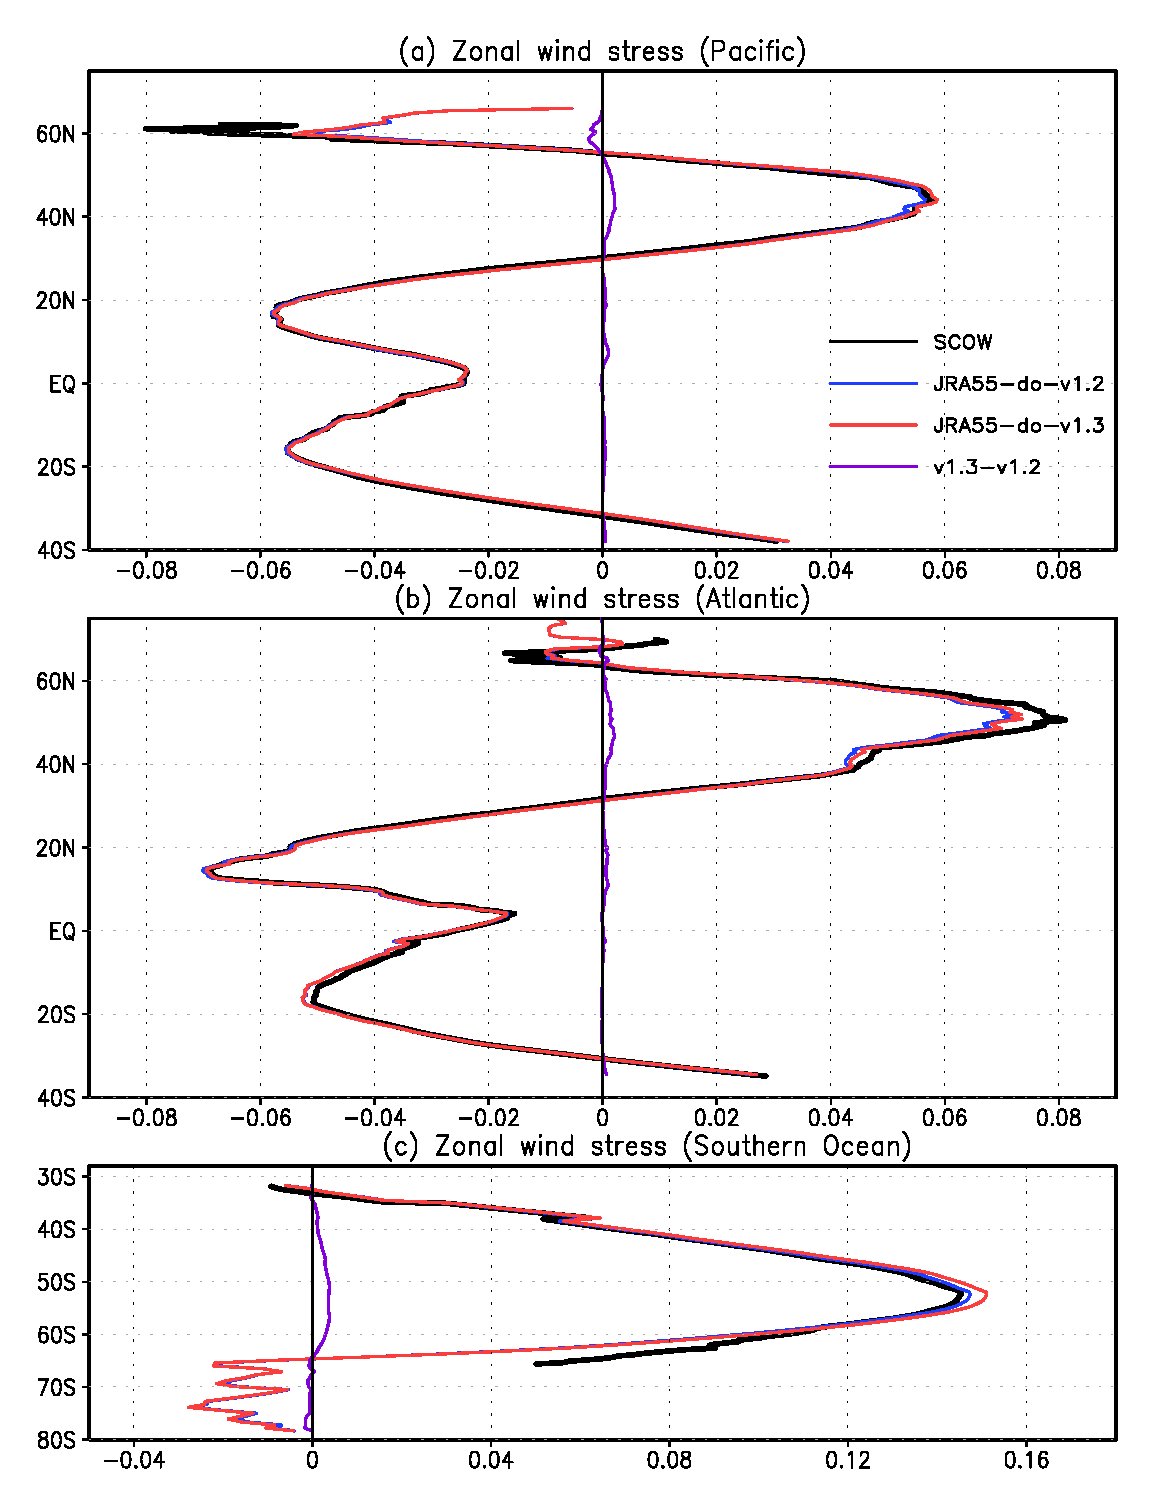
\includegraphics{taux_comp_pac_atl_scow_v1_3_prod4.eps}}
  \caption{Comparison of mean (Nov 1999 $-$ Oct 2009) basin-wide averaged zonal wind-stress ($\mathrm{N}\,\mathrm{m}^{-2}$) in (red) JRA55-do-v1.3, (blue) JRA55-do-v1.2, and (purple) difference (v1.3 - v1.2). The black lines plot the Scatterometer Oceanic Wind Stress data of \citet{Risien_and_Chelton_2008}.}
  \label{fig:taux_v1_3-v1_2}
\end{figure}

\begin{figure}[h]
  \centering
  \resizebox{!}{15cm}{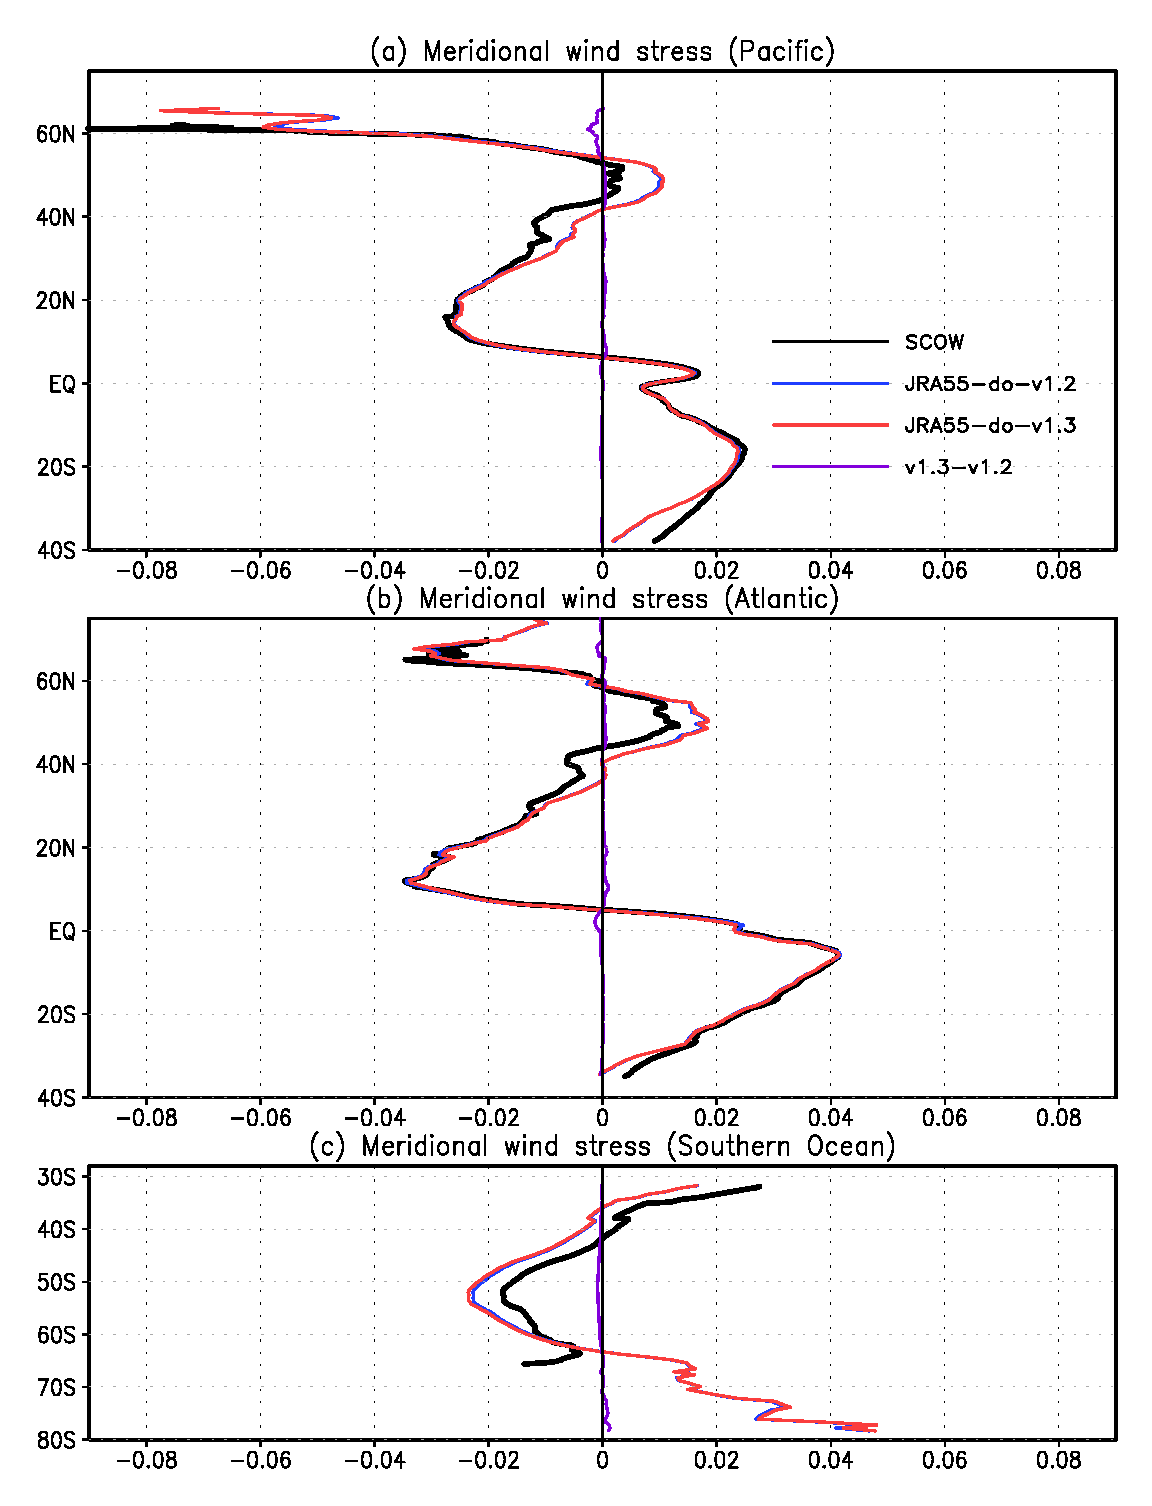
\includegraphics{tauy_comp_pac_atl_scow_v1_3_prod4.eps}}
  \caption{Same as Figure \ref{fig:taux_v1_3-v1_2} but for the meridional wind-stress.}
  \label{fig:tauy_v1_3-v1_2}
\end{figure}


\begin{figure}[h]
  \centering
  \resizebox{!}{15cm}{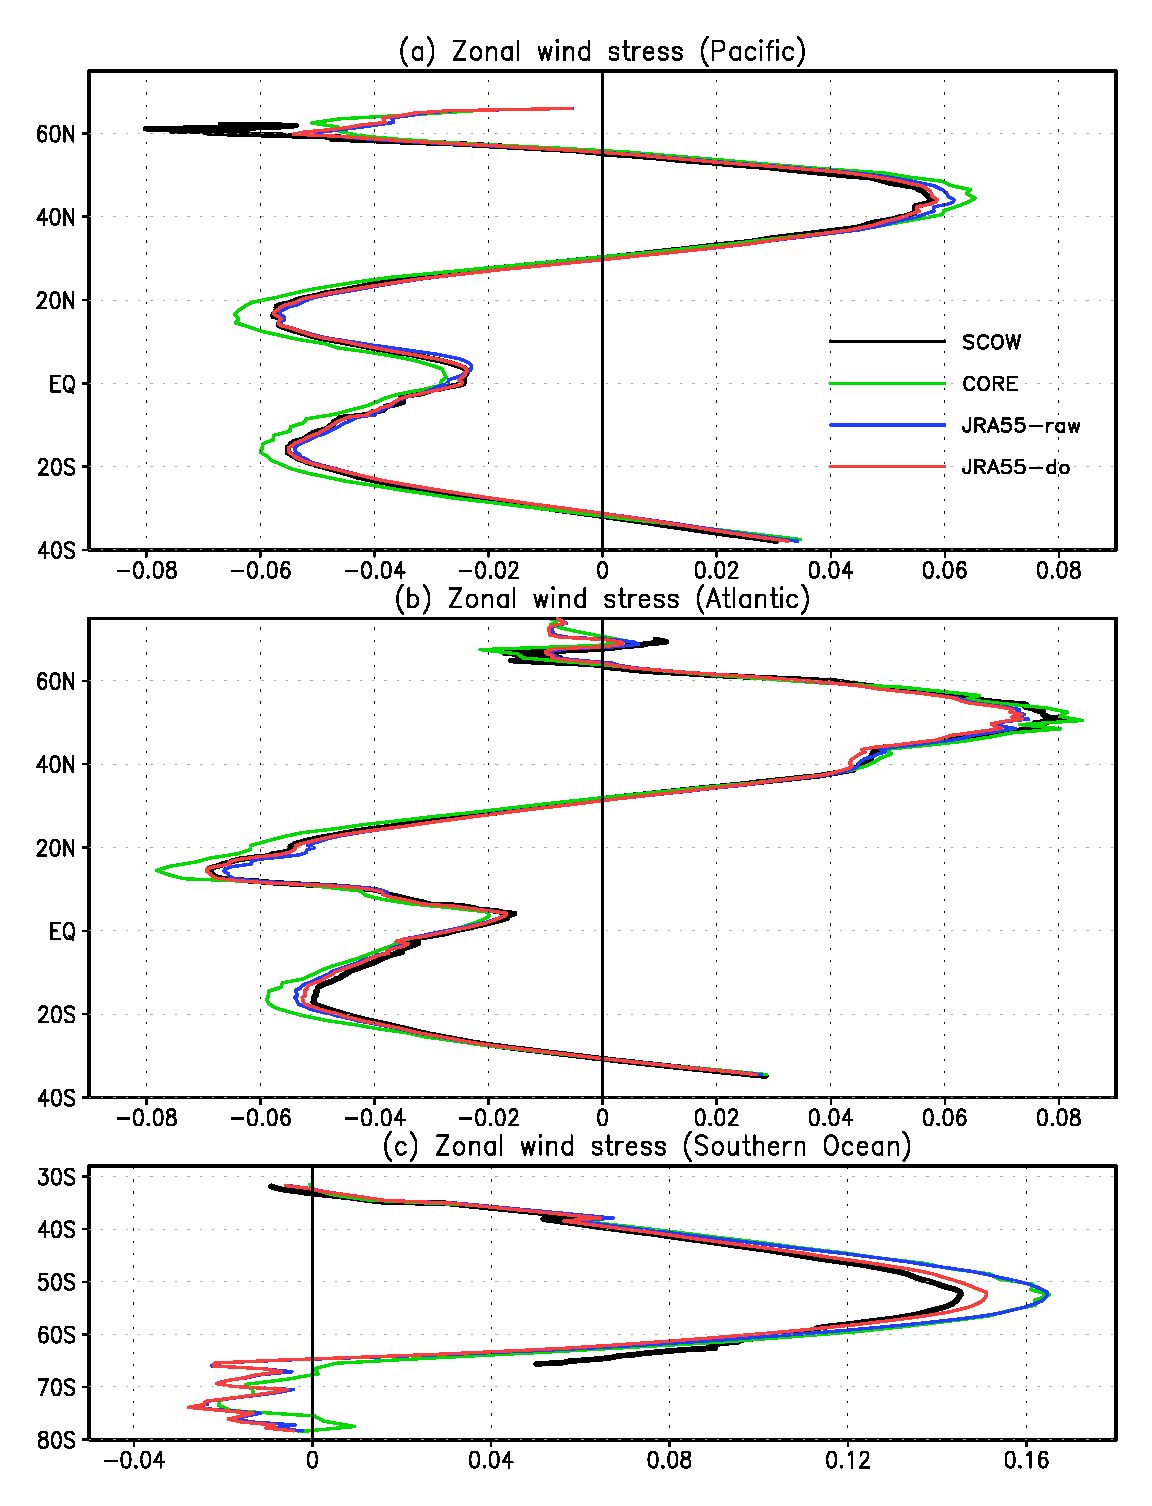
\includegraphics{taux_comp_pac_atl_scow_v1_3.eps}}
  \caption{Comparison of mean (Nov 1999 $-$ Oct 2009) basin-wide averaged zonal wind-stress ($\mathrm{N}\,\mathrm{m}^{-2}$) in (red) JRA55-do, (blue) JRA55-raw, and (green) CORE. The black lines plot the Scatterometer Oceanic Wind Stress (SCOW) data of \citet{Risien_and_Chelton_2008}. SCOW is the climatology based on September 1999 $-$ October 2009 of QuikSCAT.}
  \label{fig:comp_taux_basin}
\end{figure}

\begin{figure}[h]
  \centering
  \resizebox{!}{15cm}{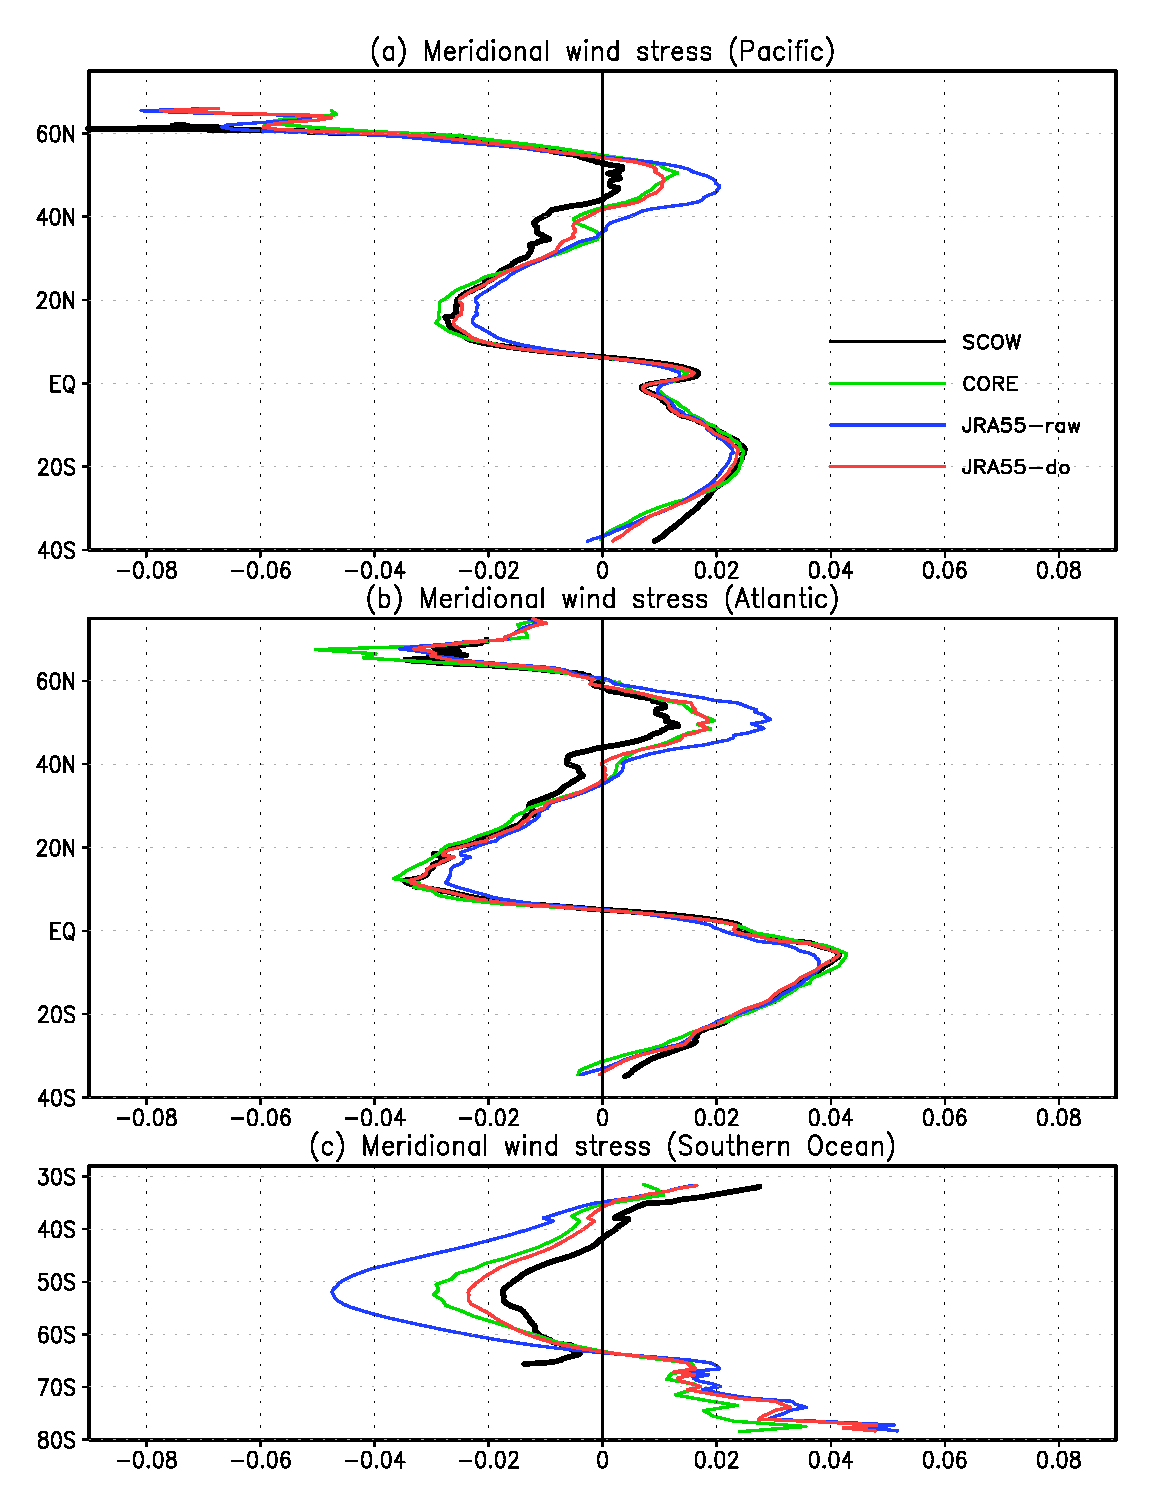
\includegraphics{tauy_comp_pac_atl_scow_v1_3.eps}}
  \caption{Same as Figure \ref{fig:comp_taux_basin} but for the meridional wind-stress.}
  \label{fig:comp_tauy_basin}
\end{figure}



\subsubsection{JRA55-do-v1.3.01 (March 2018)}
\label{app:version_1_3_1}

A bug on the cyclic condition is fixed in the smoothing scheme applied to the monthly anomaly of CORE relative to the intermediate state of the adjustment of JRA-55. Metadata and variable names are completely rewritten to comply with the convensions of the input4MIPs framework.

\begin{table}[h]
\centering
\caption{Description of the JRA55-do dataset version 1.3.1. The main variables listed here as well as supplementary data listed on Table \ref{tab:suppl_variables-1-3} can be obtained at https://esgf-node.llnl.gov/search/input4mips/. Data files are stored in netCDF format. Each file contains the annual 3-hourly and daily time-series of a single variable on the TL319 and $0.25^{\circ}\,\times\,0.25^{\circ}$ grid, for atmospheric variables and river runoff, respectively. Time-series are constructed for each year, including leap years. The first column describes the name assigned to each variable in the netCDF file. These names are taken from Climate Model Output Rewriter (CMOR). The fifth column gives the appropriate cell area in Table \ref{tab:suppl_variables-1-3} to be applied to make area averages. The sixth column gives the time of the first datum in each file. The seventh column states whether the given field is an averaged property or a snapshot. Note that rain-plus-snow equals the total precipitation. \label{tab:main_variables-1-3}}
\begin{threeparttable}
\begin{tabular*}{17.5cm}{p{1.4cm}|p{3.3cm}|p{1.6cm}|p{2.5cm}|p{1.4cm}|p{1.5cm}|p{2.8cm}}
\hline
variable name & field & units & horizontal grid cell area\tnote{5} & realm & first data represents & frequency (average or snapshot) \\ \hline \hline
$\texttt{tas}$  &  10 m air temperature   & $\mathrm{K}$ & TL319 (0.5625$^{\circ}$), $\texttt{areacello}$ & atmos & 0:00 1 Jan & 3-hour, snapshot \\ \hline
$\texttt{huss}$ &  10 m specific humidity & $\mathrm{kg}\,\mathrm{kg}^{-1}$ & TL319 (0.5625$^{\circ}$), $\texttt{areacello}$ & atmos & 0:00 1 Jan & 3-hour, snapshot \\ \hline
$\texttt{uas}$  &  10 m eastward wind     & $\mathrm{m}\,\mathrm{s}^{-1}$ & TL319 (0.5625$^{\circ}$), $\texttt{areacello}$ & atmos & 0:00 1 Jan & 3-hour, snapshot \\ \hline
$\texttt{vas}$  &  10 m northward wind    & $\mathrm{m}\,\mathrm{s}^{-1}$ & TL319 (0.5625$^{\circ}$), $\texttt{areacello}$ & atmos & 0:00 1 Jan & 3-hour, snapshot \\ \hline
$\texttt{psl}$  &  sea level pressure     & $\mathrm{Pa}$ & TL319 (0.5625$^{\circ}$), $\texttt{areacello}$ & atmos & 0:00 1 Jan & 3-hour, snapshot \\ \hline
$\texttt{rsds}$ &  downward shortwave     & $\mathrm{W}\,\mathrm{m}^{-2}$ & TL319 (0.5625$^{\circ}$), $\texttt{areacello}$ & atmos & 1:30 1 Jan & 3-hour, mean \\ \hline
$\texttt{rlds}$ &  downward longwave      & $\mathrm{W}\,\mathrm{m}^{-2}$ & TL319 (0.5625$^{\circ}$), $\texttt{areacello}$ & atmos & 1:30 1 Jan & 3-hour, mean \\ \hline
$\texttt{prra}$ & rainfall flux   & $\mathrm{kg}\,\mathrm{m}^{-2}\,\mathrm{s}^{-1}$  & TL319 (0.5625$^{\circ}$), $\texttt{areacello}$ & atmos & 1:30 1 Jan & 3-hour, mean \\ \hline
$\texttt{prsn}$ & snowfall flux   & $\mathrm{kg}\,\mathrm{m}^{-2}\,\mathrm{s}^{-1}$  & TL319 (0.5625$^{\circ}$), $\texttt{areacello}$ & atmos & 1:30 1 Jan & 3-hour, mean \\ \hline \hline
$\texttt{friver}$ & liquid water runoff\tnote{1,2,4} & $\mathrm{kg}\,\mathrm{m}^{-2}\,\mathrm{s}^{-1}$ & $0.25^{\circ}\,\times\,0.25^{\circ}$, $\texttt{areacellg}$ & ocean & 1 Jan & day, mean \\ \hline
$\texttt{licalvf}$ & solid ice runoff\tnote{3,4}  & $\mathrm{kg}\,\mathrm{m}^{-2}\,\mathrm{s}^{-1}$ & $0.25^{\circ}\,\times\,0.25^{\circ}$, $\texttt{areacellg}$ & landIce & - & year, climatology \\ \hline
\end{tabular*}
\begin{tablenotes}
 \item[1]{Data of river discharge to the ocean \citep{Suzuki_et_al_2018}, total (liquid plus solid) runoff from Greenland \citet{Bamber_et_al_2012}, and liquid water runoff from Antarctica \citep{Depoorter_et_al_2013} are merged.}
 \item[2]{There was a correction for the treatment of liquid and solid components of $\mathtt{friver}$ between version 1.3.01 and 1.3.02. See Appendix \ref{app:version_1_3_2} and Table \ref{tab:river_v1_3_2} for details.}
 \item[3]{This consists of solid ice runoff from Antarctica \citep{Depoorter_et_al_2013} represented as calving flux.}
 \item[4]{There is a major update of Greenland runoff for version 1.4. See Appendix \ref{app:version_1_4} for details.}
 \item[5]{Use the variable in this column instead of the ``cell\_measures'' attribute assigned to each variable in netCDF files.}
\end{tablenotes}
\end{threeparttable}
\end{table}

\begin{table}[h]
\centering
\caption{Description of the supplementary data of JRA55-do-v1.3.1. The first column describes the name assigned to each variable in the netCDF file. These names are taken from CMOR. \label{tab:suppl_variables-1-3}}
\begin{threeparttable}
\begin{tabular*}{17.5cm}{p{1.6cm}|p{3.3cm}|p{1.4cm}|p{2.5cm}|p{1.4cm}|p{1.5cm}|p{2.8cm}}
\hline
variable name & field & units & horizontal grid and cell area\tnote{1} & realm & first data represents & frequency (average or snapshot) \\ \hline \hline
$\texttt{ts}$   & brightness temperature from JRA-55 & $\mathrm{K}$  & TL319 (0.5625$^{\circ}$), $\texttt{areacello}$ & atmos & 0:00 1 Jan & 3-hour, snapshot \\ \hline
$\texttt{siconca}$ & sea-ice distribution from JRA-55 (0\% or 100\%) & \% & TL319 (0.5625$^{\circ}$), $\texttt{areacello}$ & seaIce & 0:00 1 Jan & 3-hour, snapshot \\ \hline
$\texttt{tos}$     & sea-surface temperature from COBE-SST \citep{Ishii_et_al_2005} & $\mathrm{^{\circ}C}$ &  1$^{\circ} \, \times \, 1^{\circ}$, n/a & ocean & 1 Jan & day, mean \\ \hline
$\texttt{siconc}$  & sea-ice distribution from COBE-SST \citep{Ishii_et_al_2005} & \% & 1$^{\circ} \, \times \, 1^{\circ}$, n/a & seaIce & 1 Jan & day, mean \\ \hline
$\texttt{sos}$ & sea-surface salinity from World Ocean Atlas 2013 v2  (\citeauthor{Zweng_et_al_2013}, \citeyear{Zweng_et_al_2013}; \citeauthor{Boyer_et_al_2015}, \citeyear{Boyer_et_al_2015}) & 0.001 & $0.25^{\circ}\,\times\,0.25^{\circ}$, $\texttt{areacellg}$ & ocean & - & month, climatology \\ \hline
$\texttt{uo}$ & sea water X velocity from GlobCurrent \citep{Rio_et_al_2014}  & $\mathrm{m}\,\mathrm{s}^{-1}$ & TL319 ($0.5625^{\circ}$), $\texttt{areacello}$ & ocean & - & year, climatology \\ \hline
$\texttt{vo}$  & sea water Y velocity from GlobCurrent \citep{Rio_et_al_2014}  & $\mathrm{m}\,\mathrm{s}^{-1}$ & TL319 ($0.5625^{\circ}$), $\texttt{areacello}$ & ocean & - & year, climatology \\ \hline \hline
$\texttt{areacello}$ & grid-cell area for surface atmospheric data & $\mathrm{m}^2$ & TL319 ($0.5625^{\circ}$), n/a & ocean & - & fixed \\ \hline
$\texttt{sftof}$ & Sea area percentage for surface atmospheric data (100\% for sea, 0\% for land) & \% & TL319 ($0.5625^{\circ}$), $\texttt{areacello}$ & ocean & - & fixed \\ \hline
$\texttt{areacellg}$ & grid-cell area for liquid water ($\mathtt{friver}$) and solid ice ($\mathtt{licalvf}$) runoff data & $\mathrm{m}^{2}$ & $0.25^{\circ} \, \times, \, 0.25^{\circ}$, n/a & landIce & - & fixed \\ \hline
\end{tabular*}
\begin{tablenotes}
 \item[1]{Use the variable in this column instead of the ``cell\_measures'' attribute assigned to each variable in netCDF files.}
\end{tablenotes}
\end{threeparttable}
\end{table}


\subsubsection{JRA55-do-v1.3.02 (March 2019)}
\label{app:version_1_3_2}

From version 1.3.02, we only update runoff data ($\mathtt{friver}$ and $\mathtt{licalvf}$) to the latest. Other variables are unchanged (except for bug fixes), but they are shifted to version 1.4 along with the upgrade of runoff from Greenland explained in Appendix \ref{app:version_1_4}.

For version 1.3.02, we corrected an error in the mapping of \citet{Bamber_et_al_2012} data on the 0.25$\times$0.25 degree runoff grid. The runoff from Greenland in the previous versions should have been shifted both westward and northward by one grid. Figure \ref{fig:bug_fix_bamber} compares the grid points where the runoff of \citet{Bamber_et_al_2012} is put in the previous and the corrected version.

Also, we corrected the definition of $\mathtt{friver}$. In version 1.3.01, $\mathtt{friver}$ represented liquid water plus solid ice runoff. However, OMIP paper \citep{Griffies_et_al_2016} defined ${\mathtt{friver}}$ as ``mass of liquid water runoff entering the ocean''. To be consistent with this definition, we corrected the data so that $\mathtt{friver}$ represents only liquid water runoff. Thus, to generate the total runoff, user must add solid ice runoff ($\mathtt{licalvf}$) to $\mathtt{friver}$. See Table \ref{tab:river_v1_3_2} for a detailed explanation.

\begin{table}[h]
\centering
\caption{Differece of $\mathtt{friver}$ between vesions 1.3.01 and 1.3.02 \label{tab:river_v1_3_2}}
\begin{threeparttable}
\begin{tabular*}{15cm}{p{2.0cm}|p{5.0cm}|p{8.0cm}}
\hline
version & field & To obtain the total runoff  \\ \hline \hline
1.3.01 & liquid water plus solid ice runoff &  Use as it is. \\ \hline
1.3.02 & liquid water runoff & Add solid ice runoff ($\mathtt{licalvf}$). \\ \hline
\end{tabular*}
\end{threeparttable}
\end{table}

\begin{figure}[h]
  \centering
  \resizebox{15cm}{!}{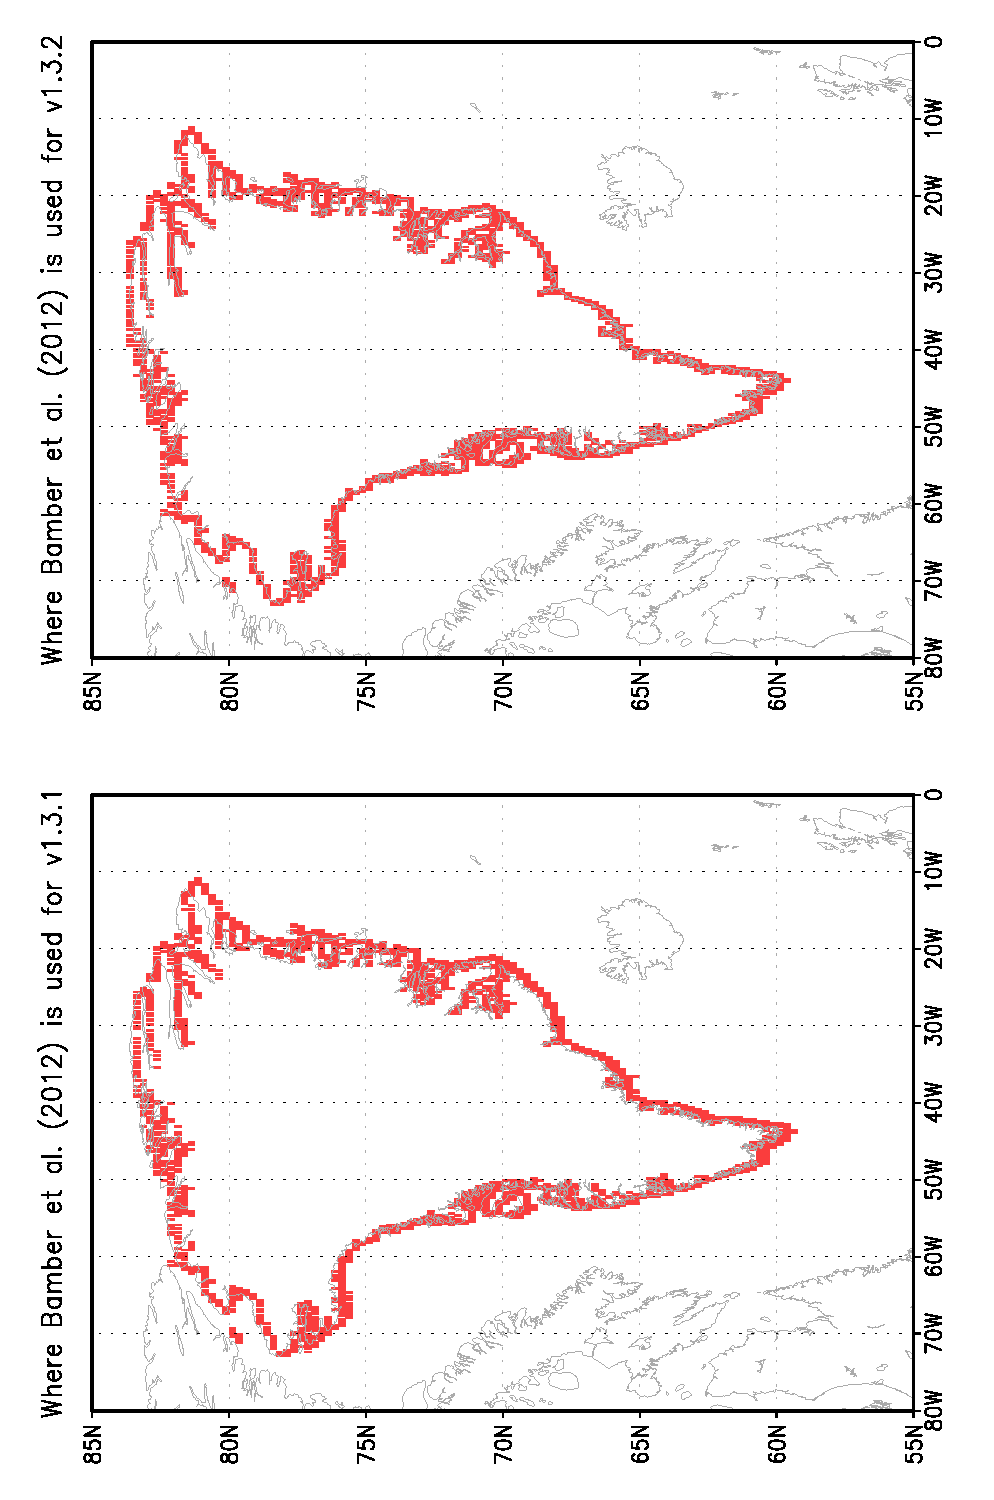
\includegraphics[angle=-90]{replace_with_bamber_2012.eps}}
  \caption{Red pixels indicate the grid points where runoff of \citet{Bamber_et_al_2012} is put in verion 1.3. (\textit{left}) Version 1.3.01 (incorrect) and (\textit{right}) version 1.3.02 (corrected).}
  \label{fig:bug_fix_bamber}
\end{figure}



\subsection{JRA55-do-v1.4 (March 2019)}

\label{app:version_1_4}

In version 1.4, we upgrade the Greenland runoff to include the time series from 1958 to 2016, as an update to \citet{Bamber_et_al_2012} that extends the seasonally-varying time series to 2016 has become available \citep{Bamber_et_al_2018}. The updated time-series also include runoff from Arctic glaciers and ice caps which have also started to rapidly lose mass since the early 2000s \citep[][]{Bamber_et_al_2018}, in addition to those over Greenland as reported by \citet{Bamber_et_al_2012}. The cumulative runoff anomaly in the new time-series is about twice that of \citet{Bamber_et_al_2012} because of the inclusion of, in particular, Canadian Arctic glaciers and the extension of the time-series to 2016. 

The daily runoff data for version 1.4 is based on the monthly runoff from 1958 to 2016 of \citet{Bamber_et_al_2018}. Time interpolation from monthly to daily data is linear. For the period before 1958 and after 2016, the monthly climatology from 1958 to 1962 and from 2012 to 2016 is used, respectively. Figure \ref{fig:replace_with_bamber} shows the grid points where the runoff from \citet{Bamber_et_al_2018} is used in place of \citet{Bamber_et_al_2012} for Greenland and \citet{Suzuki_et_al_2018} for the Canadian Arctic region, which are used in version 1.3. In version 1.4, the time series of daily solid runoff is also provided. For this data, we merge the daily solid ice runoff from Greenland based on the monthly time series of \citet{Bamber_et_al_2018} and the constant solid runoff from Antarctica \citep[][]{Depoorter_et_al_2013} which has been already used in version 1.3. Figure \ref{fig:runoff_comp_v1_3-v1_4} compares the globally integrated runoffs between versions 1.3 and 1.4. The increasing runoff of the recent decades in version 1.4 is due the use of \citet{Bamber_et_al_2018} for Greenland and the Canadian Arctic region. Table \ref{tab:main_variables_v1_4} explains the variables provided as version 1.4.

Note that the sea surface temperature ($\texttt{tos}$) has been corrected in version 1.4. The sea surface temperature of v1.3 was inappropriately subtracted by 273.15 \si{K}.

\begin{table}[h]
\centering
\caption{Description of the JRA55-do dataset version 1.4. Only runoff data are upgraded. The variables listed here can be obtained at https://esgf-node.llnl.gov/search/input4mips/. Data files are stored in netCDF format. Each file contains the annual daily time-series of a single variable on $0.25^{\circ}\,\times\,0.25^{\circ}$ grid. Time-series are constructed for each year, including leap years. The first column describes the name assigned to each variable in the netCDF file. These names are taken from Climate Model Output Rewriter (CMOR). The fifth column gives the appropriate cell area in Table \ref{tab:suppl_variables-latest} to be applied to make area averages. The sixth column gives the time of the first datum in each file. The seventh column states whether the given field is an averaged property or a snapshot. \label{tab:main_variables_v1_4}}
\begin{threeparttable}
\begin{tabular*}{17.5cm}{p{1.4cm}|p{3.3cm}|p{1.6cm}|p{2.5cm}|p{1.8cm}|p{1.5cm}|p{2.8cm}}
\hline
variable name & field & units & horizontal grid, cell area & realm & first data represents & frequency (average or snapshot) \\ \hline \hline
$\texttt{friver}$ & liquid water runoff\tnote{1} & $\mathrm{kg}\,\mathrm{m}^{-2}\,\mathrm{s}^{-1}$ & $0.25^{\circ}\,\times\,0.25^{\circ}$, $\texttt{areacellg}$ & land & 1 Jan & day, mean \\ \hline
$\texttt{licalvf}$ & solid ice runoff represented as calving flux\tnote{2} & $\mathrm{kg}\,\mathrm{m}^{-2}\,\mathrm{s}^{-1}$ & $0.25^{\circ}\,\times\,0.25^{\circ}$, $\texttt{areacellg}$ & landIce & 1 Jan & day, mean \\ \hline
\end{tabular*}
\begin{tablenotes}
\item[1]{Data of river discharge to the ocean \citep{Suzuki_et_al_2018} and liquid water runoffs around Greenland \citep{Bamber_et_al_2018} and Antarctica \citep{Depoorter_et_al_2013} are merged.}
\item[2]{Data of solid ice discharge to the ocean from Greenland \citep{Bamber_et_al_2018} and Antarctica \citep{Depoorter_et_al_2013} are merged.} 
\end{tablenotes}
\end{threeparttable}
\end{table}


\begin{figure}[h]
  \centering
  \resizebox{15cm}{!}{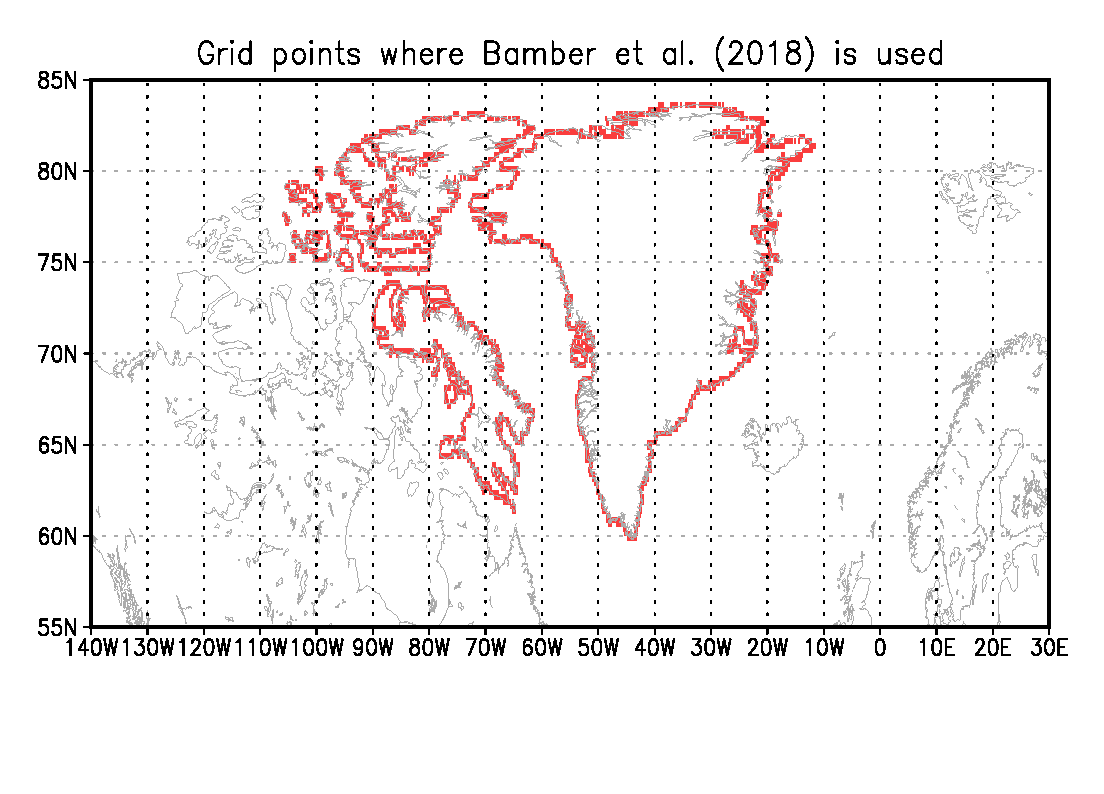
\includegraphics{replace_with_bamber_2018.eps}}
  \caption{Red pixels indicate the grid points where runoff of \citet{Bamber_et_al_2018} is used in place of that of verion 1.3.}
  \label{fig:replace_with_bamber}
\end{figure}

\begin{figure}[h]
  \centering
  \resizebox{!}{15cm}{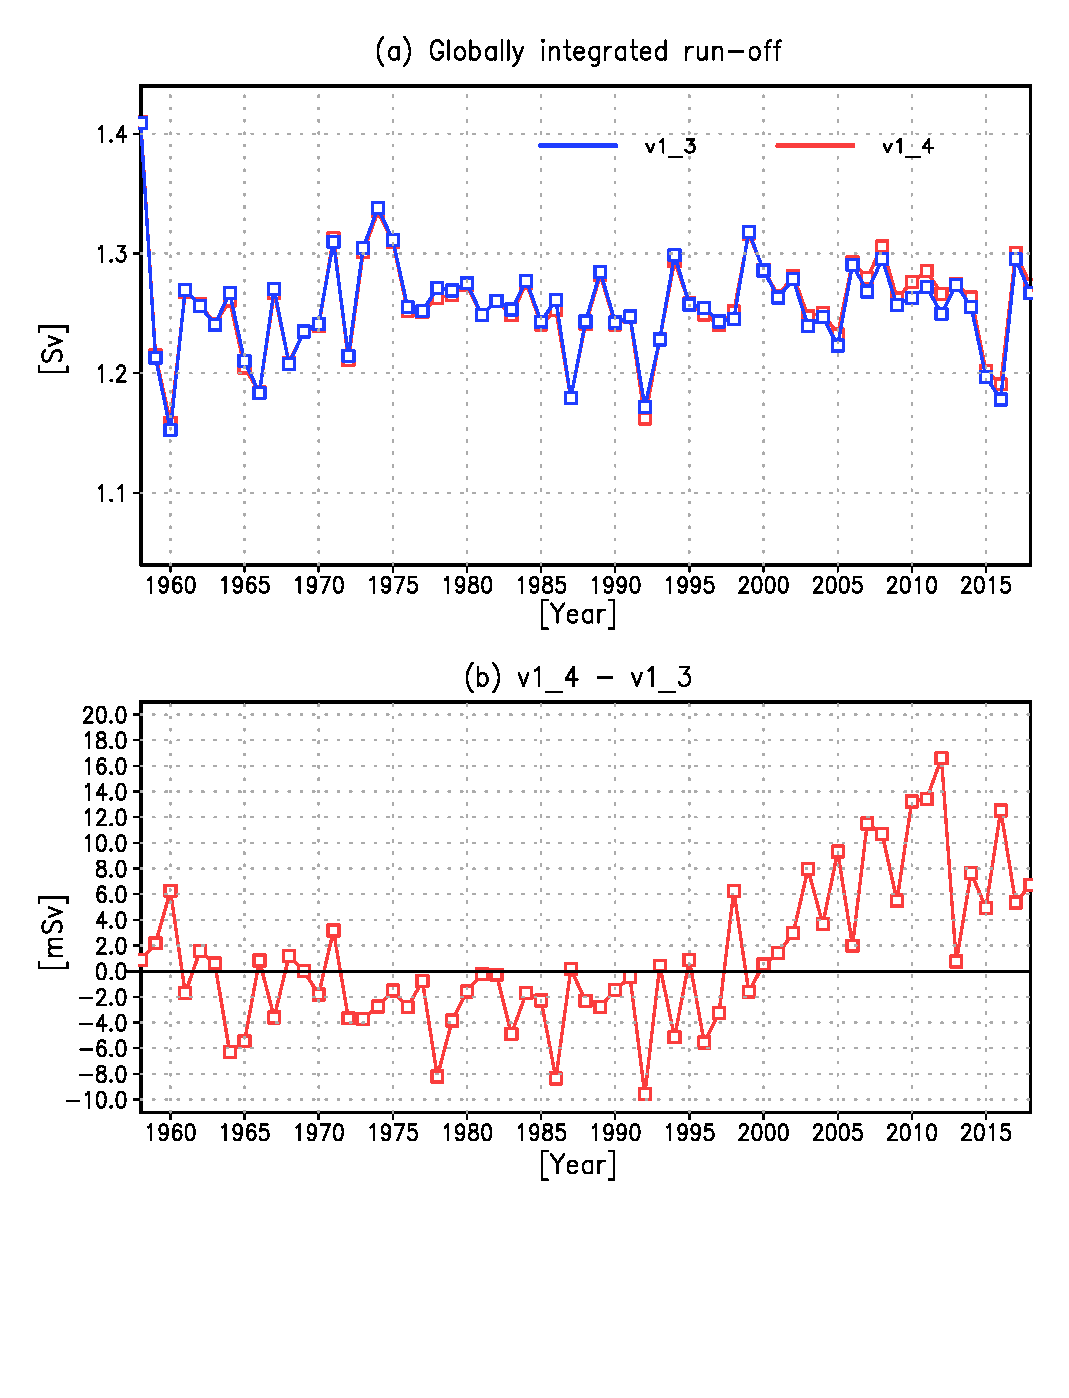
\includegraphics{runoff_comp_jra55do_v1_3-v1_4.eps}}
  \caption{(a) Globally integrated runoff ($\times 10^{9}\,\mathrm{kg}\, \mathrm{s}^{-1}$) for (blue) version 1.3 and (red) version 1.4. (b) Difference between version 1.4 and 1.3 (version 1.4 minus 1.3).}
  \label{fig:runoff_comp_v1_3-v1_4}
\end{figure}

\subsection{JRA55-do-v1.5 (September 2020)}

\label{app:version_1_5}

Version 1.5 includes the following two fixes:
\begin{itemize}
 \item The surface atmospheric fields around the erroneously (anti-cyclonically) rotating tropical cyclones that originate from the raw JRA-55 are replaced with those from 20CRv3 (\citeauthor{Slivinski_et_al_2019}~\citeyear{Slivinski_et_al_2019}). See Appendix \ref{app:version_1_5v1} for details.
 \item The surface meteorological variables (specific humidity, air temperature, and wind vector) for the period after 2016 are replaced by those based on the delayed-mode analysis of the COBE-SST dataset, instead of the real-time analysis. See Appendix \ref{app:version_1_5v2} for details.
\end{itemize}

\subsubsection{Replacement of the surface atmospheric fields around the erroneously (anti-cyclonically) rotating tropical cyclones.}
\label{app:version_1_5v1}

Erroneous behaviors are found for some tropical cyclones in the period from 1959 to 1987 in the original JRA-55 analysis. Specifically, lots of tropical cyclones have anti-cyclonic rotation in the JRA-55 analysis and the JRA55-do dataset. A report on this issue for JRA-55 can be obtained from the following.
\begin{itemize}
  \item \texttt{https://jra.kishou.go.jp/JRA-55/index\_en.html\#quality}
  \item \texttt{https://jra.kishou.go.jp/JRA-55/document/quality\_issues\_20200122\_en.pdf}
\end{itemize}

Times and positions of the erroneously represented tropical cyclones are listed in the following file.
\begin{itemize}
  \item 1959 in the Northeast Pacific: \texttt{https://jra.kishou.go.jp/JRA-55/document/anti-cyclonic\_TCs\_E\_en.txt}
  \item 1967--1987 in the North Atlantic: \texttt{https://jra.kishou.go.jp/JRA-55/document/anti-cyclonic\_TCs\_L\_en.txt}
\end{itemize}

When a tropical cyclone is erroneously analyzed, the atmospheric fields are unrealistic within a radius of approximately 1000 km from the center position for the next 6 hours of the forecast (e.g., for an erroneous analysis at 12 UTC, the forecast fields at 15 and 18 UTC are affected). Note that JRA55-do uses the forecast fields of JRA-55. This error leaves a footprint for a few days because the subsequent analyses use the forecast fields as a first guess.

Since the JRA-55 team does not have a plan to re-run the reanalysis, we have decided to replace the surface atmospheric fields around the problematic tropical cyclones of JRA55-do-v1.3 (noting that the surface atmospheric fields of JRA55-do-v1.3 and v1.4 are identical) with those from 20CRv3 (\citeauthor{Slivinski_et_al_2019}~\citeyear{Slivinski_et_al_2019}). \citet{Slivinski_et_al_2019} report that 20CRv3 is superior to similar reanalysis products (such as 20CRv2c and ERA-20C) in representing tropical cyclones. Also note that we use 20CRv3si with the prescribed SST based on SODAsi.3 before 1980 and 20CRv3mo with the prescribed SST based on HadISST2.2 after 1981 with an intention to use products prescribing more accurate SSTs. We will explain how this replacement of the surface atmospheric fields has been done in the following. Figure \ref{fig:weight_for_20CRv3}a shows the horizontal distribution of the ratio of 20CRv3 contributing to the corrected fields (JRA55-do-v1.5). The ratio is unity for 10-degree distance in geographical latitude-longitude coordinate from the center position of the erroneously analyzed tropical cyclone and the ratio decays exponentially further away with a half width of 5 degrees. This horizontal distribution is applied to the 6-hour forecast fields starting from the erroneous analysis (i.e., 3rd and 6th hour from the analysis). If a new analysis is also erroneous, the distribution of the ratio is shifted by following the new center position. After the last erroneous analysis, the horizontal distribution is kept fixed, but the ratios decay as a function of elapsed time since the last erroneous analysis time as shown in Figure \ref{fig:weight_for_20CRv3}b. From the sixth hour after the last erroneous analysis time, the weighting factor is kept unity for about 1.5 day and is gradually decreased to zero from 1.5 day to 2.5 day using a tangent hyperbolic function.

Comparison between JRA55-do-v1.3, JRA55-do-v1.5, and 20CRv3 of sea level pressure and wind vector for Tropical Cyclone 1959-10E is presented in Figure \ref{fig:1959-10E}. At 12 UTC on 21Sep1959, the tropical cyclone is normal for JRA55-do-v1.3 and JRA55-do-v1.5. From 15 UTC on 21Sep1959 to 00 UTC on 22Sep1959, the tropical cyclone rotates anti-cyclonically owing to the erroneous analyses at 12 UTC and 18 UTC on 21Sep1959. The footprint of the erroneous analysis clearly persists until about 12 UTC on 22Sep1959. During this period, 20CRv3 is used to replace those erroneous fields in JRA55-do-v1.3. The transition back to JRA55-do-v1.3 starts 24-hour later at 12 UTC on 23Sep1959 and ends approximately at 12 UTC on 24Sep1959. The tropical cyclone is well presented in JRA55-do-v1.5 by that time. In 20CRv3, the well developed cyclone is analysed only after 18 UTC on 24Sep1959. The temporal transition from 20CRv3 to JRA55-do-v1.3 from 1.5 day to 2.5 day after 6 hours from the last erroneous analysis may seem to be a conservative approach, but for some cyclones the effects of the erroneous anti-cyclonic circulation persist for about two days after the erroneous analysis. Because there are too many problematic tropical cyclones to take a case-by-case approach, we took a rather conservative approach to make the reconstruction procedure properly applied to every case.

An internal assessment using a global ocean--sea-ice model of MRI (\citeauthor{Urakawa_et_al_2020}~\citeyear{Urakawa_et_al_2020}) forced by a beta version (JRA55-do-v1.5$\beta$) that includes only the correction of surface atmospheric variables around those erroneous tropical cyclones indicates that the change in the simulated fields is largely confined near the sea surface (Figures \ref{fig:ssh-sst-v1_5-v1_4} and \ref{fig:zmts-v1_5-v1_4}) and its effect does not persist for a long time, with the differences in the annual means very small.


\begin{figure}[h]
\centering
  \resizebox{12cm}{!}{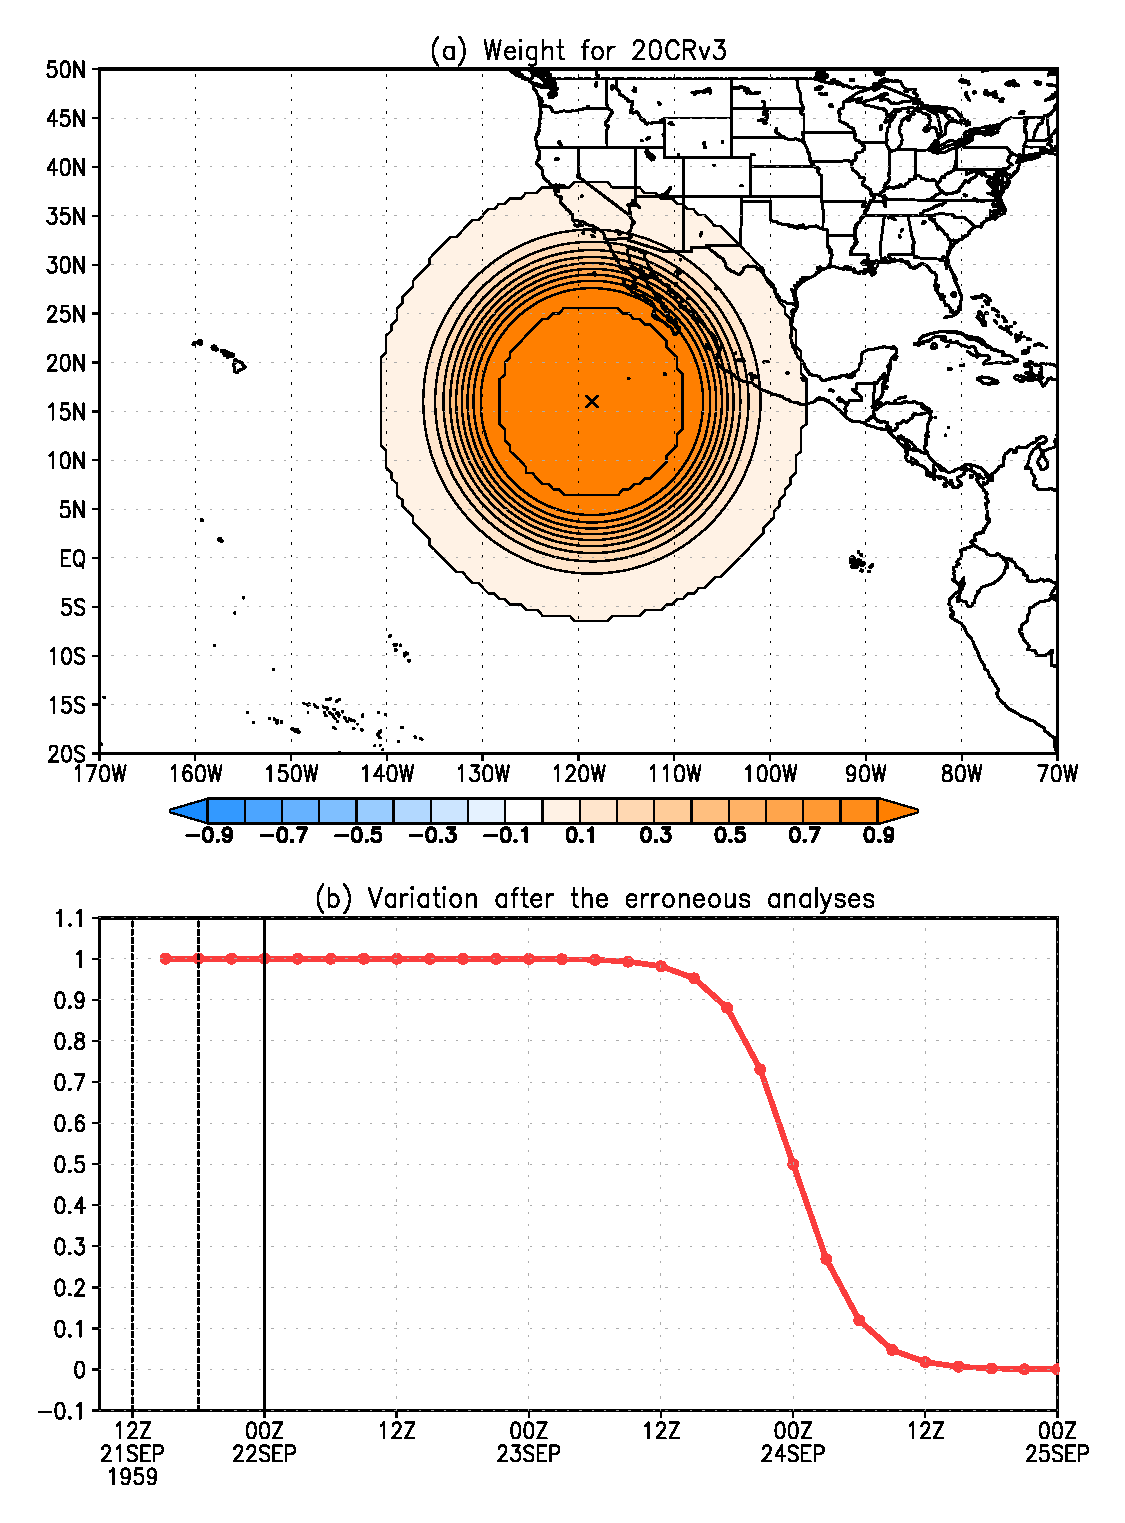
\includegraphics{v1_5/weight_20CRv3.eps}}
 \caption{An example of the ratio of 20CRv3 contributing to the surface variables of JRA55-do-v1.5. In version 1.5, surface variables around the erroneously analyzed tropical cyclones are reconstructed by merging 20CRv3 and JRA55-do-v1.3 (JRA55-do-v1.3 is identical to JRA55-do-v1.4 except for river runoff). (a) Horizontal distribution of the ratio of 20CRv3 contributing to the surface variables around the erroneously analyzed tropical cyclone (TC) 1959-10E at (16.0$^{\circ}$N, 241.4$^{\circ}$E), which is represented by the cross, at 12 UTC on 21Sep1959. This distribution is multiplied to 20CRv3 to replace part of JRA55-do-v1.3 surface atmospheric fields at 15 UTC and 18 UTC on 21Sep1959. (b) Temporal variation of the weights applied further to the ratio shown in (a). Note that TC1959-10E is erroneously analyzed at 12 and 18 UTC on 21Sep1959 (dotted vertical lines) and the erroneous analyses directly affect the forecast fields until 00 UTC on 22Sep1959 (solid vertical line). The footprint could persist up to about 2 days because the forecast fields are used as a first guess for the subsequent analyses.}
  \label{fig:weight_for_20CRv3}
\end{figure}

\begin{figure}[h]
\centering
  \resizebox{12cm}{!}{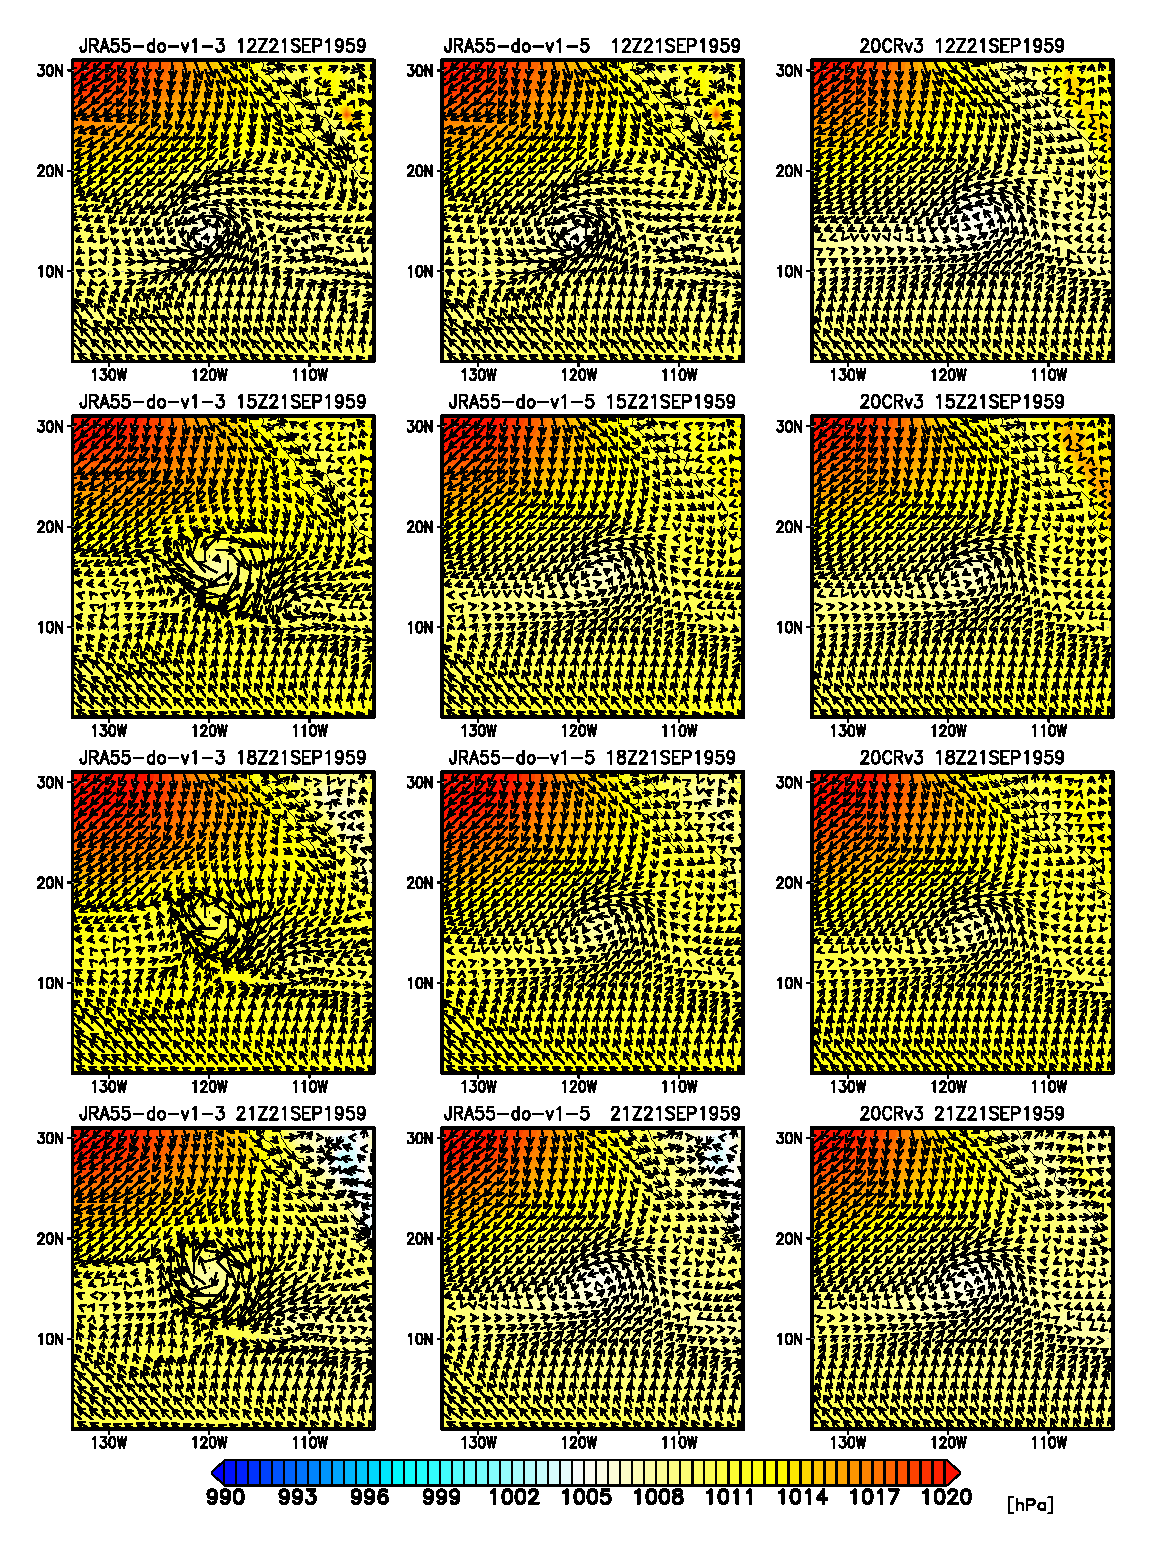
\includegraphics{v1_5/TC1959_10E/TC1959-10E-01.eps}}
 \caption{Comparison of sea level pressure and wind vector for Tropical Cyclone 1959-10E between JRA55-do-v1.3 (left), JRA55-do-v1.5 (center), and 20CRv3 (right). Snapshots with three-hour intervals from 12 UTC on 21Sep1959 to 09 UTC on 25Sep1959 are shown.}
  \label{fig:1959-10E}
\end{figure}
\setcounter{figure}{9}
\begin{figure}[h]
\centering
  \resizebox{12cm}{!}{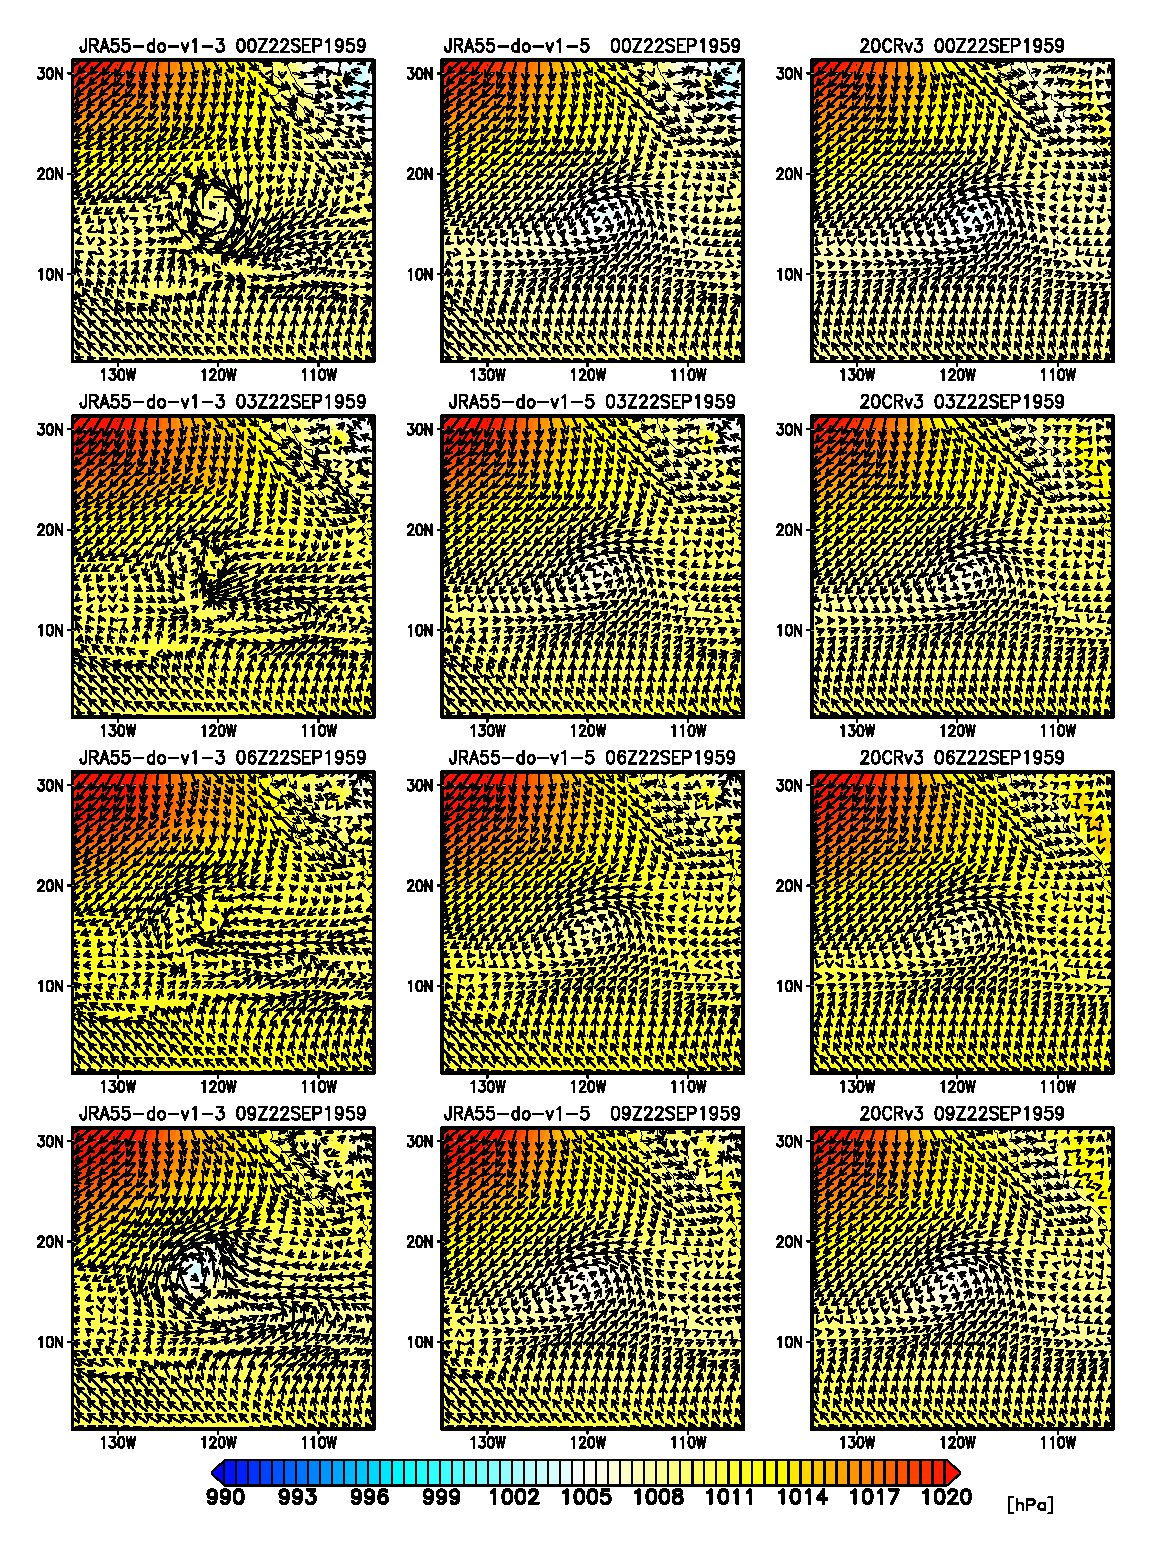
\includegraphics{v1_5/TC1959_10E/TC1959-10E-02.eps}}
  \caption{continued}
\end{figure}
\setcounter{figure}{9}
\begin{figure}[h]
\centering
  \resizebox{12cm}{!}{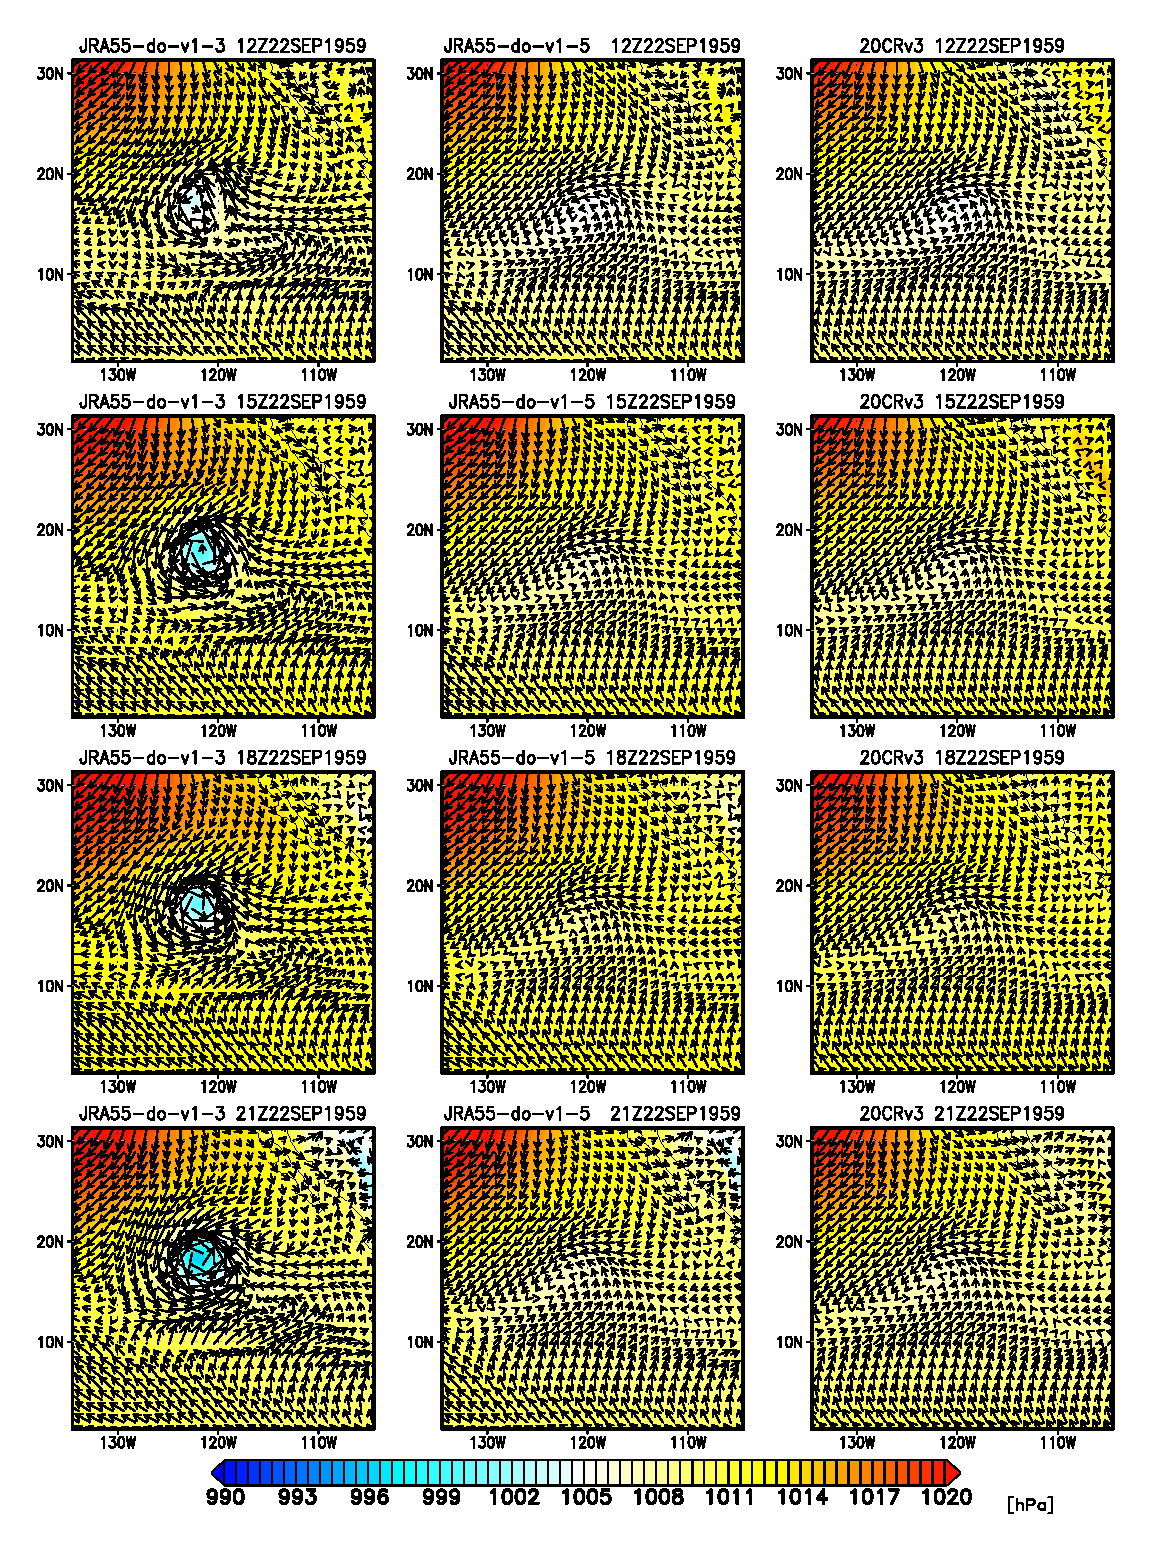
\includegraphics{v1_5/TC1959_10E/TC1959-10E-03.eps}}
  \caption{continued}
\end{figure}
\setcounter{figure}{9}
\begin{figure}[h]
\centering
  \resizebox{12cm}{!}{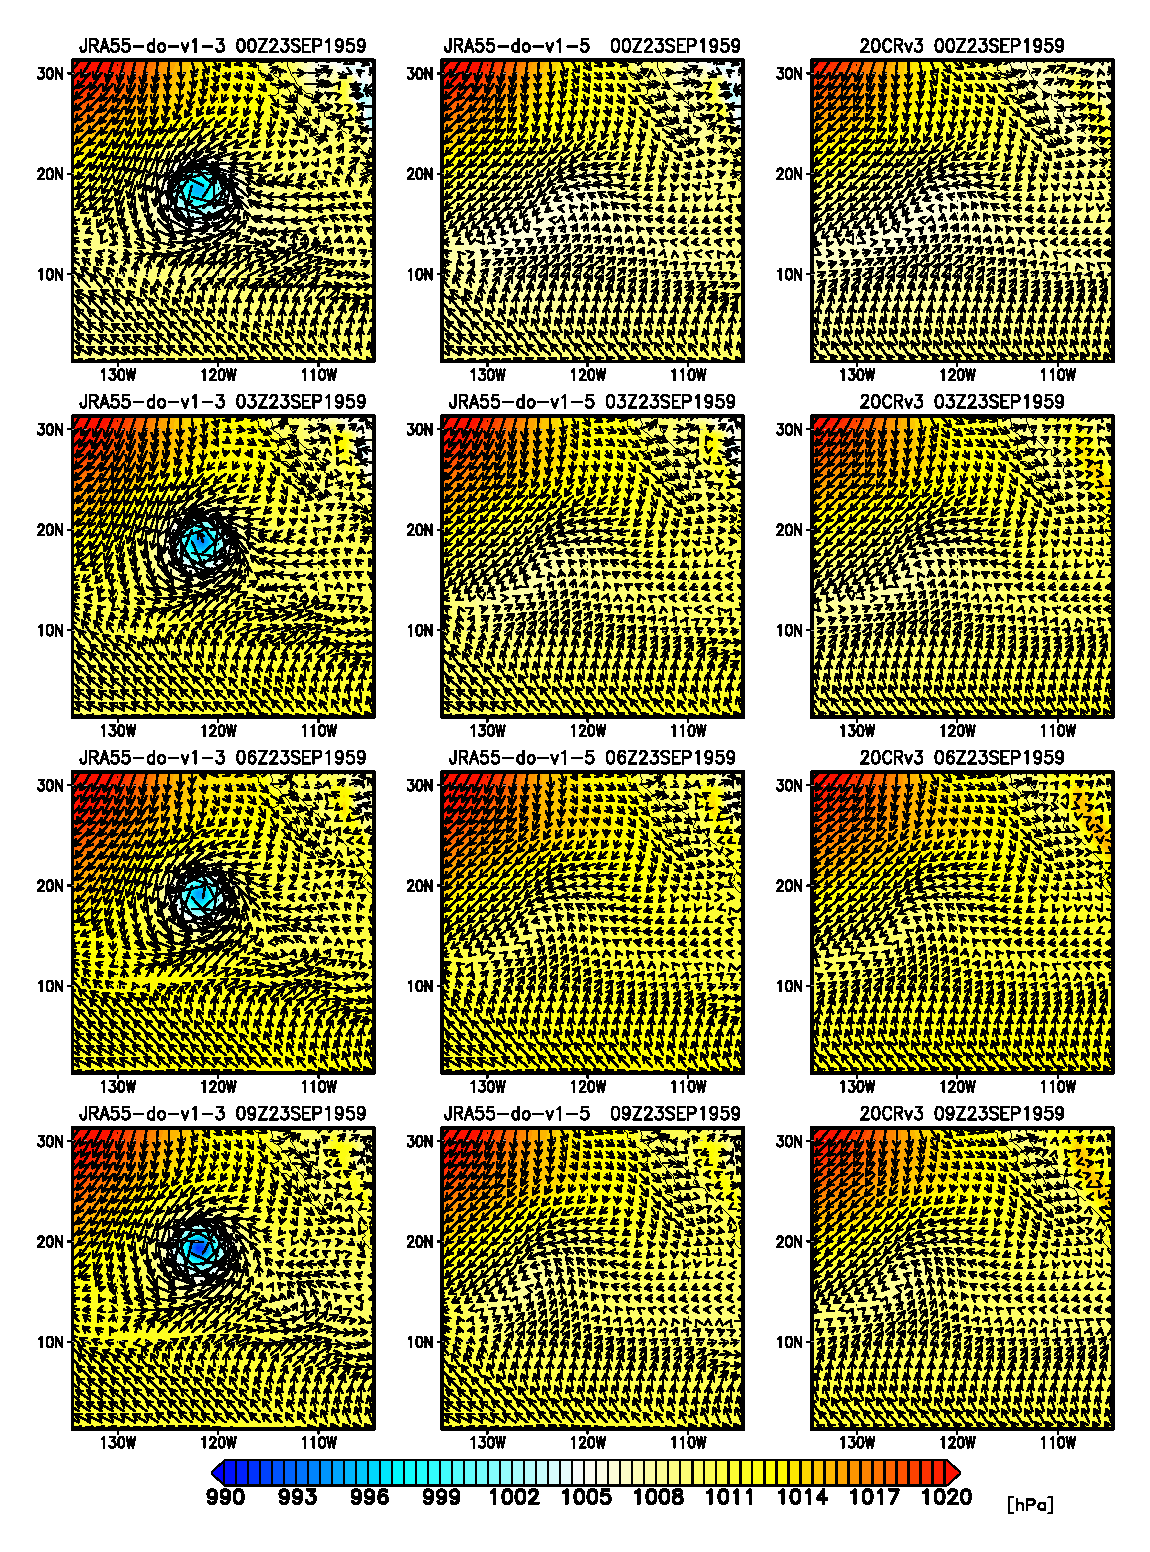
\includegraphics{v1_5/TC1959_10E/TC1959-10E-04.eps}}
  \caption{continued}
\end{figure}
\setcounter{figure}{9}
\begin{figure}[h]
\centering
  \resizebox{12cm}{!}{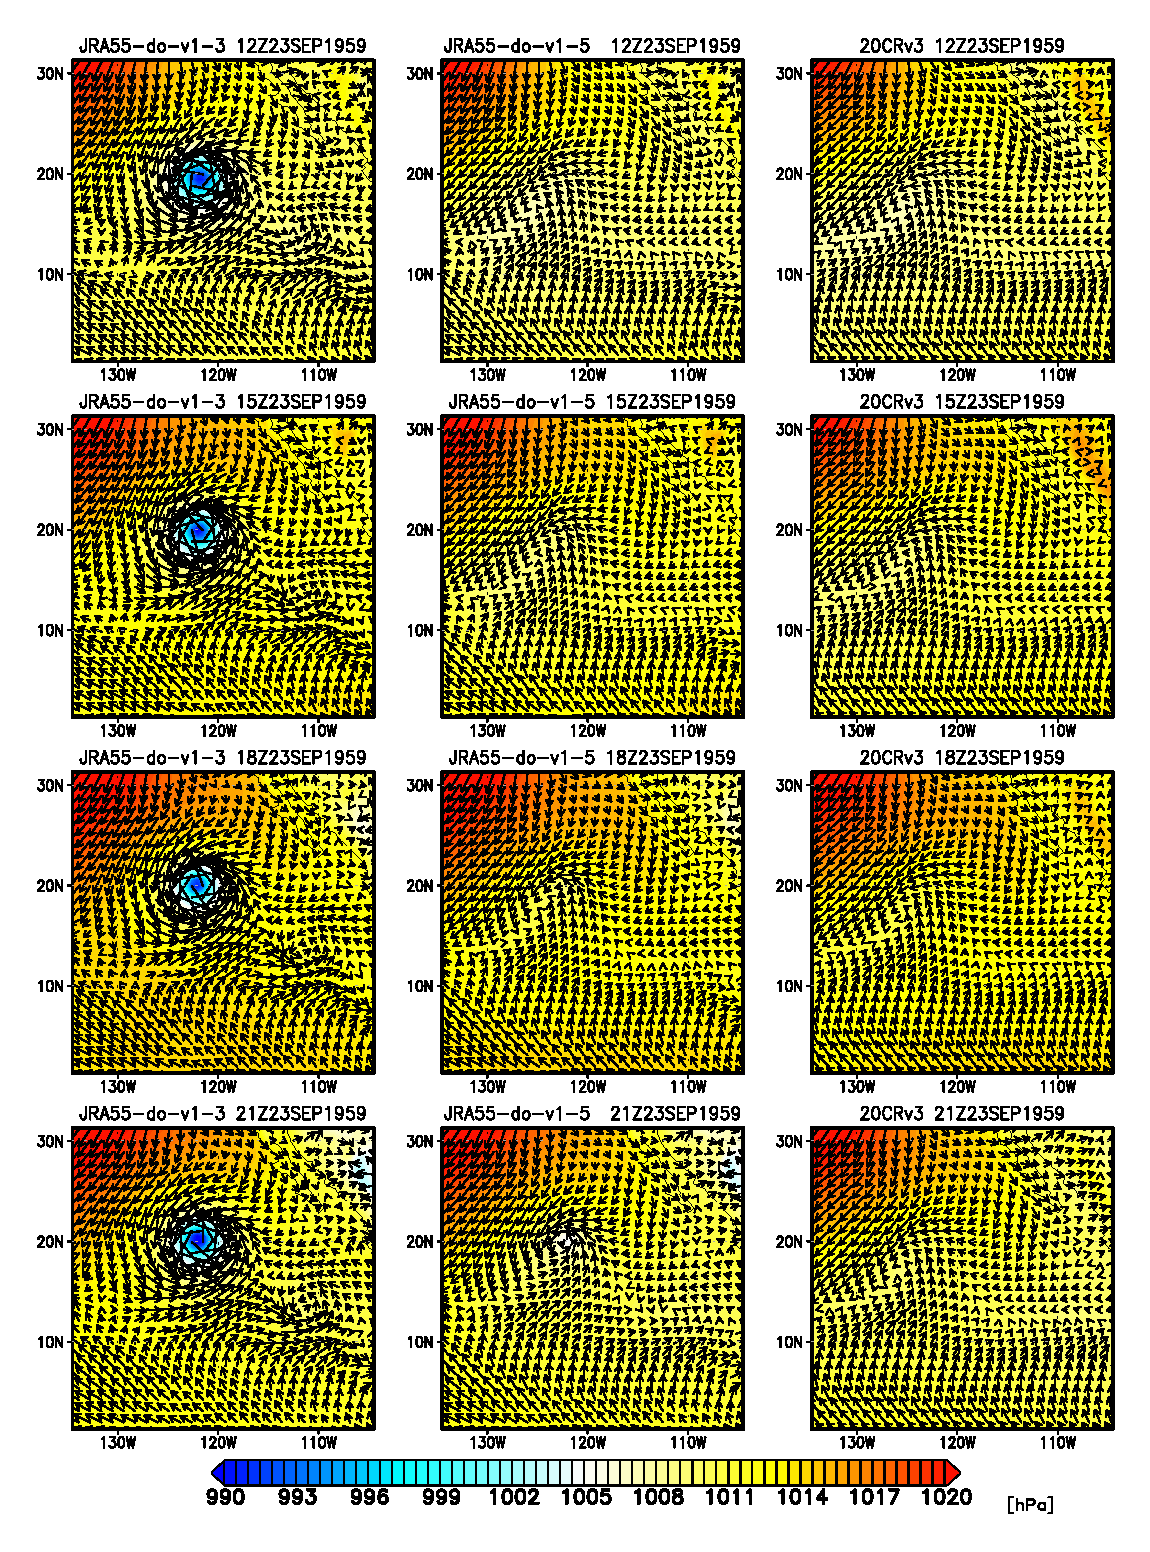
\includegraphics{v1_5/TC1959_10E/TC1959-10E-05.eps}}
  \caption{continued}
\end{figure}
\setcounter{figure}{9}
\begin{figure}[h]
\centering
  \resizebox{12cm}{!}{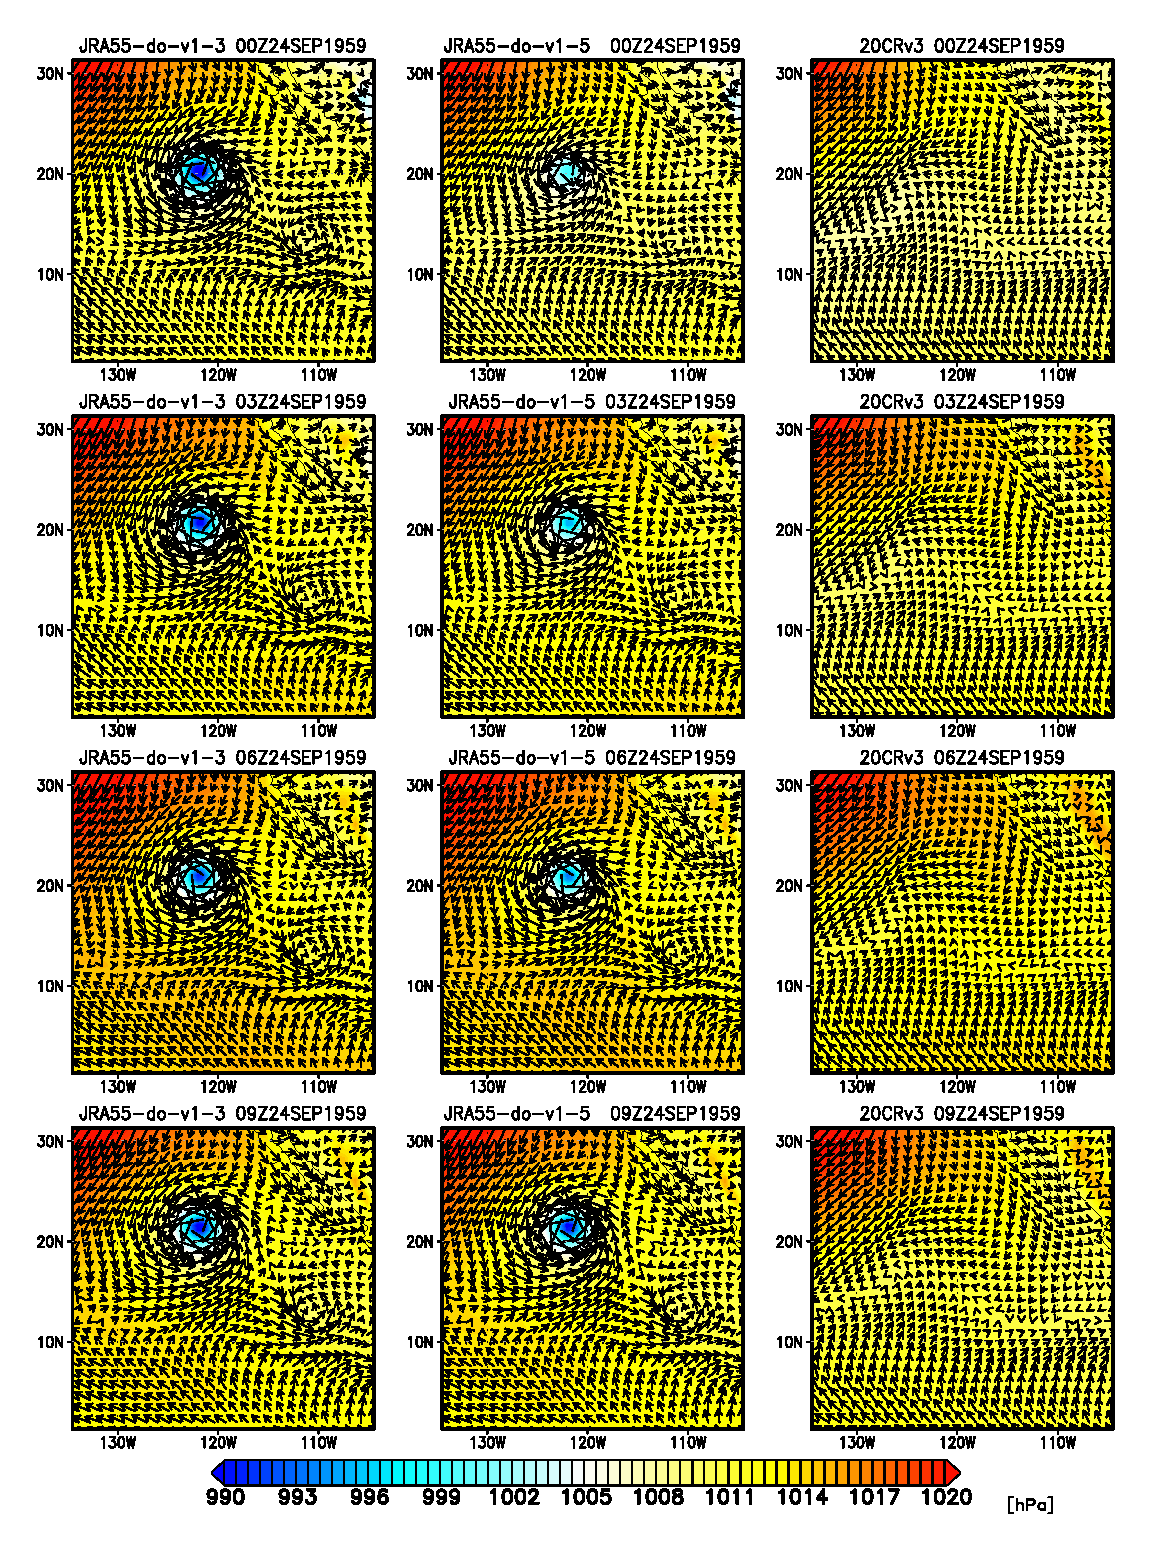
\includegraphics{v1_5/TC1959_10E/TC1959-10E-06.eps}}
  \caption{continued}
\end{figure}
\setcounter{figure}{9}
\begin{figure}[h]
\centering
  \resizebox{12cm}{!}{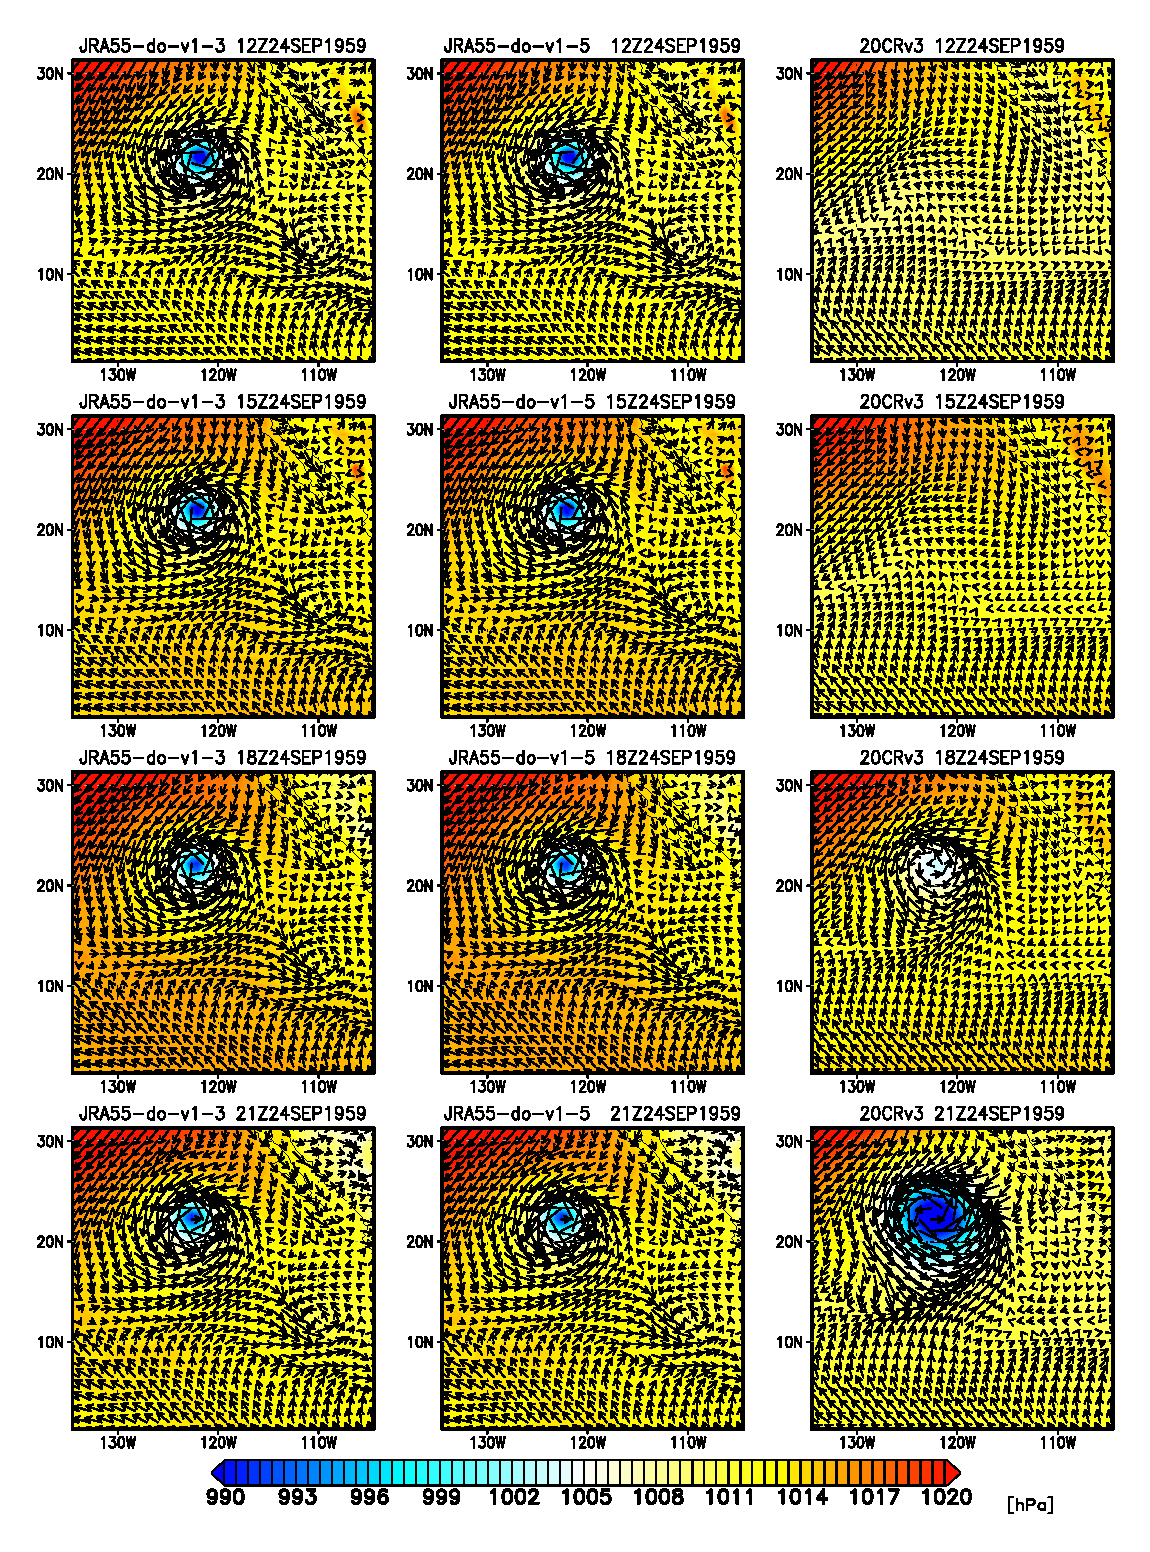
\includegraphics{v1_5/TC1959_10E/TC1959-10E-07.eps}}
  \caption{continued}
\end{figure}
\setcounter{figure}{9}
\begin{figure}[h]
\centering
  \resizebox{12cm}{!}{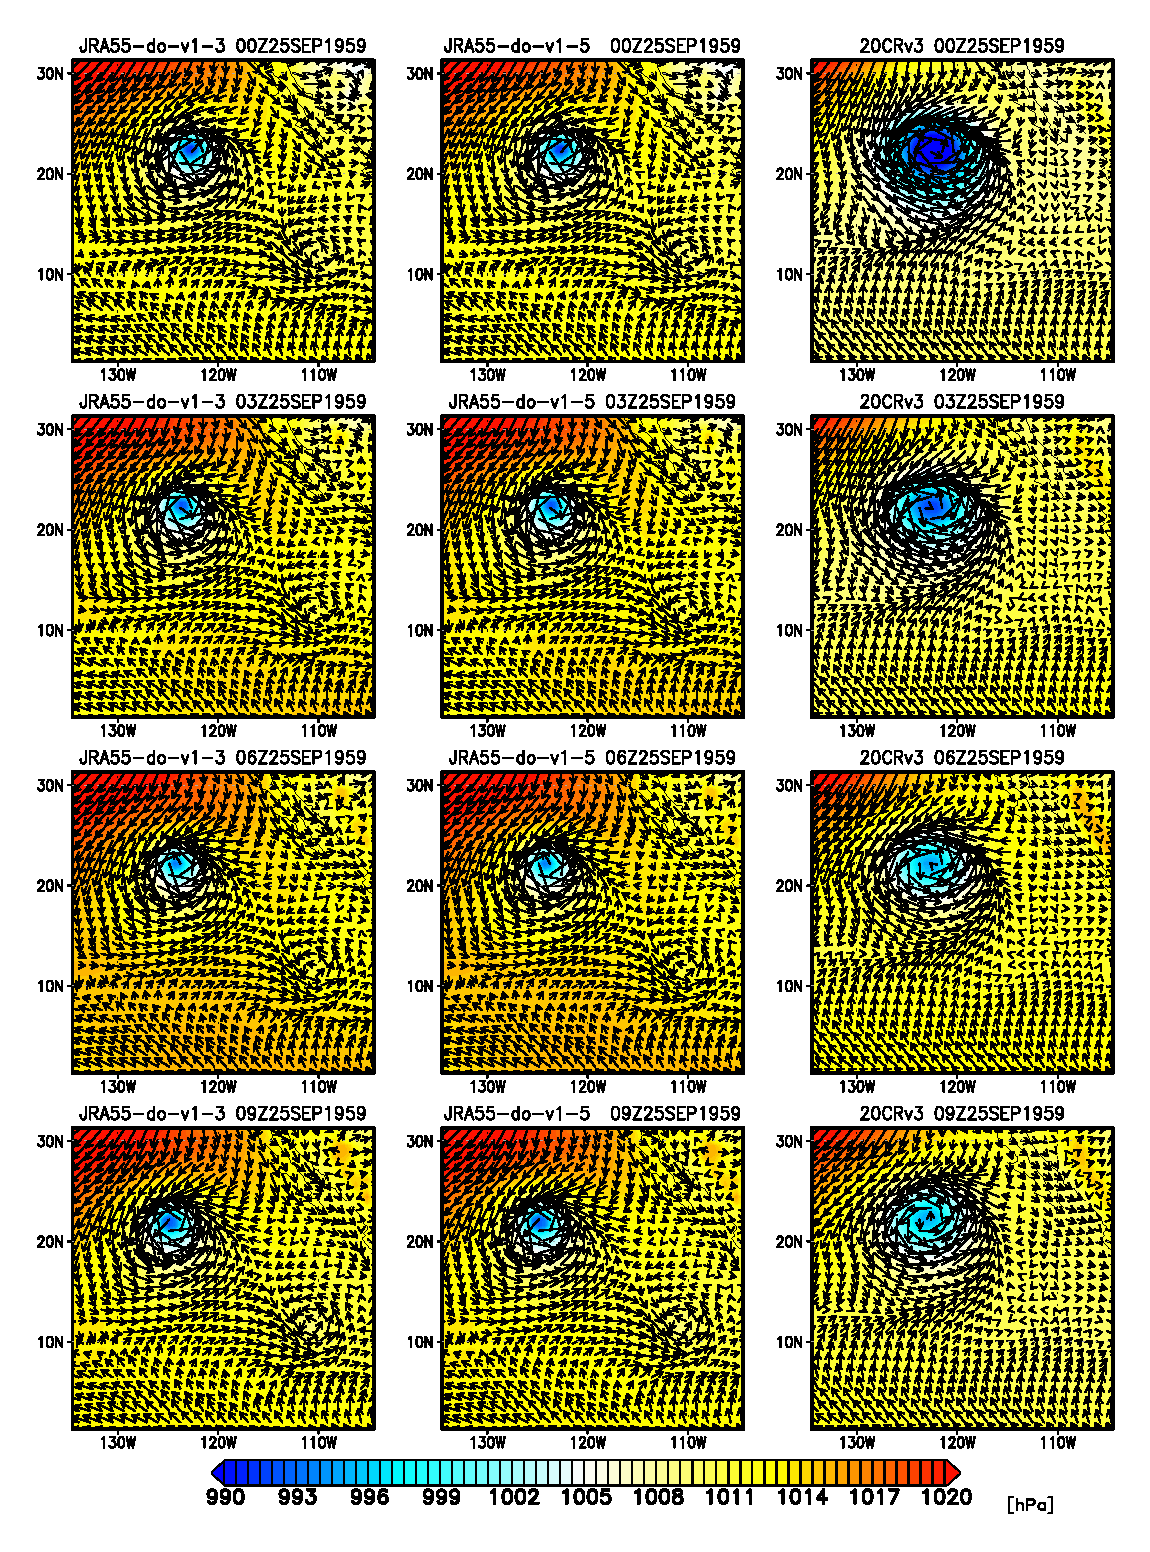
\includegraphics{v1_5/TC1959_10E/TC1959-10E-08.eps}}
  \caption{continued}
\end{figure}

\begin{figure}[h]
\centering
  \resizebox{12cm}{!}{\includegraphics{v1_5/ssh-sst_diff1967-1967.eps}}
 \caption{Difference between the simulations of a global model of MRI (\citeauthor{Urakawa_et_al_2020}~\citeyear{Urakawa_et_al_2020}) forced by v1.5$\beta$ and v1.4 (v1.5$\beta$ minus v1.4). Annual mean (a) sea surface height and (b) sea surface temperature in the year 1967, when many tropical cyclones in the North Atlantic are erroneously analyzed in JRA-55. Note that v1.5$\beta$ includes only corrections for surface atmospheric variables around the erroneously analyzed tropical cyclones.}
  \label{fig:ssh-sst-v1_5-v1_4}
\end{figure}

\begin{figure}[h]
\centering
  \resizebox{12cm}{!}{\includegraphics{v1_5/zmt_diff_cyc_1967-1967.eps}}
  \caption{Difference between the simulations of a global model of MRI (\citeauthor{Urakawa_et_al_2020}~\citeyear{Urakawa_et_al_2020}) forced by v1.5$\beta$ and v1.4 (v1.5$\beta$ minus v1.4). Annual mean basin wide averaged (a) temperature and (b) salinity in the year 1967.}
  \label{fig:zmts-v1_5-v1_4}
\end{figure}

\begin{figure}[h]
\centering
  \resizebox{14cm}{!}{\includegraphics[angle=-90]{v1_5/ts_amoc_diff_org_1653-2018.eps}}
  \caption{Comparison between the simulations of a global model of MRI (\citeauthor{Urakawa_et_al_2020}~\citeyear{Urakawa_et_al_2020}) forced by v1.5 and v1.4 for the entire integration period (6-cycles of the 61-year (1958-2018) JRA55-do forcing). Atlantic meridional overturning circulation maximum at 26$^{\circ}$N (a) and its difference (v1.5 minus v1.4) (b). Units are Sverdrups (1 Sverdrup = 10$^{9}\,\mathrm{kg}\,\mathrm{s}^{-1}$). Globally averaged temperature (c) and its difference (v1.5 minus v1.4) (d). Units are $^{\circ}$C. In (a) and (c), blue lines are used for v1.5 and red lines are used for v1.4. Since differences are very small as shown in (b) and (d), only red lines (v1.4) are discernible.}
  \label{fig:amoc-ts-v1_5-v1_4}
\end{figure}

\subsubsection{Use of the delayed-mode analysis of COBE-SST for the period from 2016 to present.}
\label{app:version_1_5v2}

For the years after 2016 of the previous versions, the COBE-SST data based on the real-time analysis had been used as the lower boundary condition in the processing of surface atmospheric variables using the bulk formula. On the other hand, for years before 2016, the COBE-SST data based on the delayed-mode analysis had been used for processing. For each daily COBE-SST data, the delayed-mode data becomes available about one month later, overwriting the existing real-time data. This means that only the set of delayed-mode data is available for later analyses. To ensure the consistency and the reproducibility of the entire dataset, all meteorological variables processed using COBE-SST, specifically surface air temperature, specific humidity, and wind vector, have been recalculated using the delayed-mode COBE-SST for years after 2016. The data in the following periods were based on the real-time analysis of COBE-SST and thus were replaced by the new data based on the delayed mode COBE-SST:
\begin{itemize}
 \item 15:00 5 Dec 2016 -- 09:00 1 Jan 2017,
 \item 15:00 3 Dec 2017 -- 09:00 1 Jan 2018,
 \item 15:00 3 Dec 2018 -- 09:00 1 Jan 2019,
 \item 15:00 15 Dec 2019 -- 09:00 1 Jan 2020.
\end{itemize}
The first date that the difference arises changes year to year. This is because the dates when COBE-SST was obtained for processing data of the previous year in January of a new year were different.

The overall effect of this correction is considered minor. As shown in Figure \ref{fig:amoc-ts-v1_5-v1_4}, large scale circulation metrics such as A-MOC and global mean ocean temperature are almost unchanged between simulations forced by JRA55-do-v1.4 and JRA55-do-v1.5.

As an additional note, we treat the data created with the delayed-mode COBE-SST as the final product. In v1.5.0.1 that extends v1.5.0 to latest, the surface meteorological variables (specific humidity, air temperature, and wind vector) for the lastest 30 days are preliminary because they are adjusted using the real-time analysis of the COBE-SST dataset. They are sequentially (day-by-day) replaced by final ones as the delayed-mode analysis of the COBE-SST dataset becomes available.

\section*{Acknowledgments}

Authors are grateful to Sasha Ames in LLNL and Martina Stockhause in DKRZ for their technical supports in making the dataset available from input4MIPs and Karl Taylor in LLNL for various advice on the generation of datasets with high integrity. They are also grateful to Masayoshi Ishii in MRI for providing computation resources. The feedback and supports provided by Patrik Hyder at UK Met Office, Kazutoshi Oonogi and Masahiro Hosaka at MRI, and participants of \textit{CLIVAR Ocean Model Development Panel (OMDP) Mini Workshop on Forcing Ocean--Sea-ice Models}, which was held in January 2015 in Grenoble, France, \textit{Extended CLIVAR-OMDP panel meeting on forcing ocean-ice climate models}, which was held in January 2016 in Yokohama, Japan, and CLIVAR OMDP panel meetings, which were held in September 2016 in Qingdao, China and in October 2017 in Exeter, UK, and the continuous support from the members of CLIVAR-OMDP as well as the many other modelling groups that have tested versions of JRA55-do, are gratefully acknowledged.

COBE-SST, WOA13v2, and GlobCurrent products were obtained from the following cites:\\
 \hspace*{3zw} COBE-SST: https://ds.data.jma.go.jp/tcc/tcc/products/elnino/cobesst/cobe-sst.html.\\
 \hspace*{3zw} WOA13v2: https://www.nodc.noaa.gov/OC5/woa13/woa13data.html.\\
 \hspace*{3zw} GlobCurrent products: http://globcurrent.ifremer.fr/.

The development of the JRA55-do dataset is supported by JSPS KAKENHI Grant Number 15H03726. NCAR contribution to this study is supported by the NOAA Climate Program Office Climate Variability and Predictability Program.

The present effort to produce the JRA55-do dataset is a project separated from the JRA-55 project conducted by Japan Meteorological Agency. Feedback should be directed to the authors of this document, not to the contact of the JRA-55 project.

%\clearpage

\section*{References}

\bibliography{User_manual_jra55_do_v1_5}

\end{document}
